\documentclass[a4paper,12pt]{scrartcl}
\usepackage[utf8]{inputenc}
\usepackage[ngerman]{babel}
\usepackage[T1]{fontenc}
\usepackage[left= 3.5cm,right = 3cm, bottom = 4 cm, top = 2.5cm]{geometry}
\usepackage[onehalfspacing]{setspace}
%\usepackage{here}
%\usepackage{float}
\usepackage[ngerman]{cleveref}
\usepackage[table]{xcolor}
%\usepackage{acronym}
%\usepackage{mcode/mcode}
% ============= Packages =============

% Dokumentinformationen

%\usepackage{hyperref} % ermöglicht Hyperlinks in PDF-Dokumenten
%definecolor{LinkColor}{rgb}{0,0,0}
%\hypersetup
%	{
	% Farbein der Verweise
%	             colorlinks, % farbige Links anstelle von Boxen
	% Farben für Bildschirmanzeige
	%            linkcolor=red, % Farbe für normale interne Links
	%            anchorcolor=black, % Farbe für Ankertext
	%            citecolor=green, % Farbe für bibliografische Zitate im Text
	%            filecolor=magenta, % Farbe für URLs auf lokale Dateien
	%            menucolor=red, % Farbe für Acrobat-Menü-Elemente
	%            urlcolor=cyan, % Farbe für URLs
	% Farben für Druck
%	             linkcolor=black, % Farbe für normale interne Links
%	             anchorcolor=black, % Farbe für Ankertext
%	             citecolor=black, % Farbe für bibliografische Zitate im Text
%	             filecolor=black, % Farbe für URLs auf lokale Dateien
%	             menucolor=black, % Farbe für Acrobat-Menü-Elemente
%	             urlcolor=black, % Farbe für URLs
	%            linkcolor=blue, % Farbe für normale interne Links
	%            anchorcolor=black, % Farbe für Ankertext
	%            citecolor=green, % Farbe für bibliografische Zitate im Text
	%            filecolor=magenta, % Farbe für URLs auf lokale Dateien
	%            menucolor=red, % Farbe für Acrobat-Menü-Elemente
	%            urlcolor=blue, % Farbe für URLs
	% PDF Metadaten
%	             pdftitle={Türklingelnanlage mit Standardkomponente }, % Titel des PDF Dokuments
%	             pdfauthor={Federico Crameri, Geo Bontognali}, % Verfasser des PDF Dokuments
	%            pdfsubject={}, % Thema des PDF Dokuments
	%            pdfkeywords={}, % Stichwörter des PDF Dokuments
%	             pdfdisplaydoctitle=true, % Titel anstelle Dateinamen in Titelzeile anzeigen
%	}


% Standard Packages
\usepackage{graphicx}
%\usepackage{subfigure}
\usepackage{fancyhdr}
\usepackage{lmodern}
%\usepackage{color}
%\usepackage{transparent}
%\usepackage{tabu}
%\usepackage{siunitx}
%\usepackage{here}
%\usepackage{tikz}
%\usepackage{caption} 
%\usepackage{slashed}
%\usepackage{cancel}
\usepackage{multicol}
\usepackage{tabularx}
%\usepackage{adjustbox}
%\usepackage{wallpaper}
%\usepackage{transparent}

%\usepackage[style=authortitle-icomp]{biblatex} 
%\bibliography{C:\Users\Gabriel\Desktop\Bachelorarbeit\Fachmodul\Bericht\literatur} 

%\sisetup{detect-weight=true, detect-family=true}

\graphicspath{{img/}}

% Aufzählung Packages
%\usepackage{paralist}

% Tabellen Packages
%\usepackage{booktabs}
\usepackage{multirow}
%\usepackage{cite}
%\usepackage{multibib}

% zusätzliche Schriftzeichen der American Mathematical Society
\usepackage{amsfonts}
\usepackage{amsmath}
%\usepackage{mathtools}
%Grad Zeichen
%\usepackage{textcomp}
%\usepackage{courier}

% nicht einrücken nach Absatz
\setlength{\parindent}{0pt}

% Literaturverzeichnis
\usepackage{url}

% ========================== Kopf- und Fußzeile =======================================
\pagestyle{fancy}
%
\lhead{} %\thepage
%\chead{}
\rhead{\slshape \leftmark}
%%
\lfoot{}
\cfoot{\thepage}
\rfoot{}

%%
\renewcommand{\headrulewidth}{0.4pt}
\renewcommand{\footrulewidth}{0pt}

% ========================== Package Einstellungen & Sonstiges ========================== 

%Besondere Trennungen

%römische Aufzählungen mit \RM{Zahl}
\newcommand{\RM}[1]{\MakeUppercase{\romannumeral #1}}
\newcommand{\MATLAB}{\textsc{Matlab}\xspace}

\newcommand{\seeref}[1]{\seename \ \cref{#1}}

\renewcommand{\theequation}{\thesection.\arabic{equation}}


% ======================================= Dokumentbeginn =======================================

\begin{document}


\pagestyle{empty}
\begin{titlepage}
%\ThisTileWallPaper{\paperwidth}{\paperheight}{image/Titleimage.png}


	\begin{flushleft}
		
\includegraphics[scale=0.1]{image/ntb.jpg}
	\end{flushleft}
	
    \begin{center}
	    \vspace{1cm}
	    \Huge \textbf{\textsf{Türklingelanlage mit Standardkomponenten}} \\
		\vspace{1cm}
		\large\textbf{\textsc{Federico Crameri, Geo Bontognali}}\\
		
		\vspace{1cm}
	    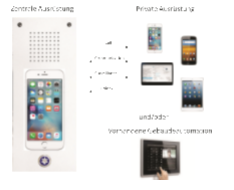
\includegraphics[height=8cm]{image/Titleimage.png}
	
	    \normalsize
	    \vspace{1cm}
	    \large \textbf{Bachelorarbeit}\\
	    \vspace{1cm}
	
	 \normalsize
	 	{
			\begin{tabular}{lll}
				\textbf{Studiengang:} & & Systemtechnik\\
				\textbf{Profil:} & & Informations- und Kommunikationssysteme\\
				\textbf{Referent:} & & Prof. Dr. Hauser-Ehninger Ulrich, MSc in Electronic Engineering\\
				\textbf{Korreferent:} & & Toggenburger Lukas, Master of Science FHO in Engineering\\
			\end{tabular}
	    }
    \end{center}
\end{titlepage}

\cleardoublepage
% \part im Inhaltsverzeichnis nicht nummerieren
\makeatletter
\let\partbackup\l@part
\renewcommand*\l@part[2]{\partbackup{#1}{}}

% leere Seite einfügen nach dem Titel
\thispagestyle{empty}
\quad 
\newpage

\pagenumbering{Roman}
\pagestyle{plain}
\section*{Zusammenfassung}
\label{sec:zusammenfassung}
%\addcontentsline{toc}{section}{Zusammenfassung}

Lorem ipsum dolor sit amet, consetetur sadipscing elitr, sed diam nonumy eirmod tempor invidunt ut labore et dolore magna aliquyam erat, sed diam voluptua. At vero eos et accusam et justo duo dolores et ea rebum. Stet clita kasd gubergren, no sea takimata sanctus est Lorem ipsum dolor sit amet. Lorem ipsum dolor sit amet, consetetur sadipscing elitr, sed diam nonumy eirmod tempor invidunt ut labore et dolore magna aliquyam erat, sed diam voluptua. At vero eos et accusam et justo duo dolores et ea rebum. Stet clita kasd gubergren, no sea takimata sanctus est Lorem ipsum dolor sit amet. Lorem ipsum dolor sit amet, consetetur sadipscing elitr, sed diam nonumy eirmod tempor invidunt ut labore et dolore magna aliquyam erat, sed diam voluptua. At vero eos et accusam et justo duo dolores et ea rebum. Stet clita kasd gubergren, no sea takimata sanctus est Lorem ipsum dolor sit amet.   

Duis autem vel eum iriure dolor in hendrerit in vulputate velit esse molestie consequat, vel illum dolore eu feugiat nulla facilisis at vero eros et accumsan et iusto odio dignissim qui blandit praesent luptatum zzril delenit augue duis dolore te feugait nulla facilisi. Lorem ipsum dolor sit amet, consectetuer adipiscing elit, sed diam nonummy nibh euismod tincidunt ut laoreet dolore magna aliquam erat volutpat.   

Ut wisi enim ad minim veniam, quis nostrud exerci tation ullamcorper suscipit lobortis nisl ut aliquip ex ea commodo consequat. Duis autem vel eum iriure dolor in hendrerit in vulputate velit esse molestie consequat, vel illum dolore eu feugiat nulla facilisis at vero eros et accumsan et iusto odio dignissim qui blandit praesent luptatum zzril delenit augue duis dolore te feugait nulla facilisi.   

Nam liber tempor cum soluta nobis eleifend option congue nihil imperdiet doming id quod mazim placerat facer

\section*{Abstract}
\label{sec:abstract}
%\addcontentsline{toc}{section}{Abstract}

In a world where everything is moving forward at the speed of light, home building technology is no exception. There are plenty of systems needed around building a house. One of them is the intercom.   
\\
\\
During our bachelor thesis, we developed a prototype for an intercom, based on open source software and hardware components. One of the aims of this project, was to evaluate and proof the ability of such components to handle this kind of application.
\\
During the design phase, many different requirements were defined. The intercom needed to be able to provide an audio and video stream. Nowadays everyone is always connected to the internet, thanks to the power of modern communication systems like Tablets and Smartphones. So, there was no doubt about the need of the intercom to be fully digital. As soon as things like digital real-time Video- and Audio transmissions comes on the table, also a lot of different complications and challenges comes with it too.
\\
\\
As a result, we came up with a prototype, that provides a flexible, up-to-date, and reasonably inexpensive solution for a modern house intercom system.

\newpage

% leere Seite einfügen
\thispagestyle{empty}
\quad 
\newpage
%%Inhaltsverzeichnis
\tableofcontents
\newpage

%%Seitennummerierung neu beginnen, Zahlen [arabic], röm.Zahlen [roman,Roman], Buchstaben [alph,Alph]
\pagenumbering{arabic}
\newpage
\pagestyle{fancy}






%\section{Einleitung}
\label{sec:einleitung}

List Example:
\begin{itemize}
\item Maximaler Schub beim Starten z.B. wegen kurzer Startbahn
\item Maximale Fluggeschwindigkeit erreichen z.B. bei Rettungsflügen oder Ähnlichem
\item Maximale Effizienz z.B. um möglichst lange Flugzeiten zu ermöglichen
\end{itemize}



Bild Beispiel:
\vspace{0.05cm}

\begin{figure}[htb!]
	\begin{center}
		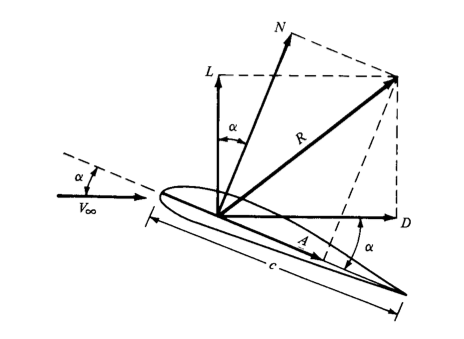
\includegraphics[width=0.48\textwidth]{airfoilKraefte}
		\caption[Wirksame aerodynamische Kräfte an einem Profil]{Wirksame aerodynamische Kräfte an einem Profil \cite{aeroKraefte}. Die Auftriebskraft $L$ wirkt beim Propeller als Schub und die Widerstandskraft $D$ als Drehmoment.}
		\label{fig:airfoilKraefte}
	\end{center}
\end{figure}

\vspace{0.05cm}

Unterkapittel:

\subsection{Subsection test}
\label{subsec:speichernderresultatematlab}

Wenn die Propellerberechnung beendet ist, werden alle Resultate in eine Baumstruktur gespeichert. Somit sind die Resultate schnell wieder aufrufbar und auch sauber in einer einzigen Datei geordnet und gespeichert.\\

\subsubsection{Subsubsection test}
\label{subsubsec:speichernderresultatematla2}

Wenn die Propellerberechnung beendet ist, werden alle Resultate in eine Baumstruktur gespeichert. Somit sind die Resultate schnell wieder aufrufbar und auch sauber in einer einzigen Datei geordnet und gespeichert.\\

\subsubsection{Subsubsubsection test}
\label{subsubsec:speichernderresultatematlab3}

Wenn die Propellerberechnung beendet ist, werden alle Resultate in eine Baumstruktur gespeichert. Somit sind die Resultate schnell wieder aufrufbar und auch sauber in einer einzigen Datei geordnet und gespeichert.\\

\newpage


%\section{Chapter Example}
\label{sec:chapterexample}


Um Berechnungen rund um das Thema Propeller durchführen zu können, ist es nötig, die sogenannte Blade- und Momentum-Theorie zu verstehen und diese anwenden zu können. Die Ausführungen in dieser Arbeit orientieren sich stark an der Master-Thesis von Mario Heene\cite{heene}. Ebenfalls werden die wichtigsten Begriffe der Aerodynamik und Propellertheorie erläutert. 
%\subsection{Underchapter Example}
\label{subsec:underchapterexample}

Die Gestalt von Propellern kann durch viele 2D-Profile beschrieben werden. 2D-Profile gleichen dem Querschnitt eines Flügels. Durch den geringeren Druck auf der Oberseite des Profils resultieren Kräfte, die das Profil hoch drücken (siehe Kapitel \ref{subsec:momentumtheorie}, Einschub Bernoulli) oder im Falle des Propellers, Schub erzeugen. Für jedes Profil können die Kräfte dargestellt werden.

\vspace{0.05cm}

\begin{figure}[htb!]
\begin{center}
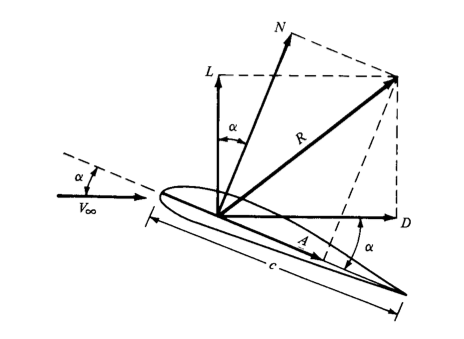
\includegraphics[width=0.48\textwidth]{airfoilKraefte}
\caption[Wirksame aerodynamische Kräfte an einem Profil]{Wirksame aerodynamische Kräfte an einem Profil \cite{aeroKraefte}. Die Auftriebskraft $L$ wirkt beim Propeller als Schub und die Widerstandskraft $D$ als Drehmoment.}
\label{fig:airfoilKraefte}
\end{center}
\end{figure}

\vspace{0.05cm}

In Abbildung \ref{fig:airfoilKraefte} sind die verschiedenen Kräfte dargestellt. $V_\infty$ stellt die Geschwindigkeit der Luft weit weg vom Körper dar. Die Kraft $R$ setzt sich zusammen aus der Auftriebskraft $L$ ('lift') und der Widerstandskraft $D$ ('drag'), wobei $L$ senkrecht zu $V_\infty$ steht und $D$ in die gleiche Richtung zeigt wie $V_\infty$.
Die Sehnenlänge $c$ ('chord') definiert die Länge des Profils von der Profilspitze bis zur Hinterkante. Dabei steht die Kraft $N$ senkrecht zu $c$ und $A$ in Richtung $c$. Der Winkel $\alpha$ ist der Winkel zwischen $V_\infty$ und $c$.
Über trigonometrische Funktionen können die Kräfte $N$ und $A$ folgendermassen beschrieben werden:

 

\section{Einführung}
\label{sec:chapterexample}

\subsection{Problemstellung}
\label{sec:chapterexample}

Heutzutage liefern diverse Hersteller verschiedene Lösungen für das Türglockensystem. Diese sind meistens Komplettsysteme, die nicht nur das einfache Klingel ermöglichen, sondern auch Zusatzfunktionen wie das Video-Streaming anbieten. Diese Systeme sind aber meistens proprietär und werden, gemäß Abschnitt \ref{sec:marktsituation},  für sehr hohe Preise verkauft.
\\
Die Komponenten, die für solche Systeme notwendig sind, sind aber heutzutage kostengünstig auf dem Markt erhältlich. Das Erarbeiten preiswerter Lösungen müsste somit möglich sein.
\\
Natürlich spielen die Kosten einer \gls{turklingelanlage} auf die Investitionen eines Neubaus keine so grosse Rolle. Sicher besteht aber in diesem Bereich eine Marktlücke und somit die Möglichkeit neue, bessere und günstigere Lösungen zu entwickeln.

\subsection{Grundidee}
\label{sec:grundidee}
Die Grundidee dieser Arbeit ist es, durch das Zusammenspiel verschiedener Systemen und Technologien, eine kostengünstige und funktionale \gls{turklingelanlage} zu entwickeln.
\\ 
Um den Kostenfaktor zu berücksichtigen, soll die Anlage auf schon vorhandene Technologien und Hardware basieren. Somit fallen die hohen Kosten für die Beschaffung proprietärer Hardware weg.
\\
In einer Zeit, in der die Hausautomation und das «Internet of things» immer mehr Bedeutung gewinnen, soll die \gls{turklingelanlage} diese Standards in Betracht ziehen. Dieses System soll den Benutzern ermöglichen, Ihre \gls{turklingelanlage} durch herkömmliche Smartphone oder Tablet zu bedienen.
\\
Klingelt ein Besucher an der Eingangstüre, soll der Wohnungsbesitzer über sein Smartphone darauf aufmerksam gemacht werden. Über eine am Eingang installierte Kamera  bekommt er auch die Möglichkeit den Besucher im Streaming zu sehen und die Türe, falls erwünscht, durch einen Handybefehl zu öffnen.
\newpage

\section{Projektplanung}
\label{sec:chapterexample}

\subsection{Prozess}
\label{sec:chapterexample}
Als Entwicklungsprozess wird ein hybrides Vorgehensmodell eingesetzt, welcher in Abbildung \ref{fig:hybridesModell} dargestellt wird. Im Rahmen einer Bachelorarbeit, in der die Anforderungen und Analysen schon im voraus im Fachmodul definiert worden sind, eignet sich am bestens ein lineares V-Modell. Ein solcher Prozess ist sehr schlank, übersichtlich und für diese Projektgrösse geeignet.
\\
Was das V-Modell nicht erlaubt, ist eine ständige Iteration mit dem Kunden während der Entwurf/Implementierungsphase. Daraus ergibt sich, wie im Abbild unten gezeigt, ein hybrides Modell welches uns zulässt, trotz der klar definierten Anforderungen, während der Entwurf- und der Implementierungsphase ein agiles Vorgehen mit dem Kunden durchzuführen.
\\
Die im Fachmodul geleistete Arbeit gehört zu den ersten zwei Phasen des Modells. Wie im linearen Vorgehensmodell vorgegeben, beginnt die nächste Phase der Arbeit sobald die vorherige Phase abgeschlossen ist. Die ganze Bachelorarbeit basiert auf Evaluationen und Entscheidungen, die in den ersten Phasen des Projekts getroffen worden sind. 

\begin{figure}[htb!]
	\begin{center}
		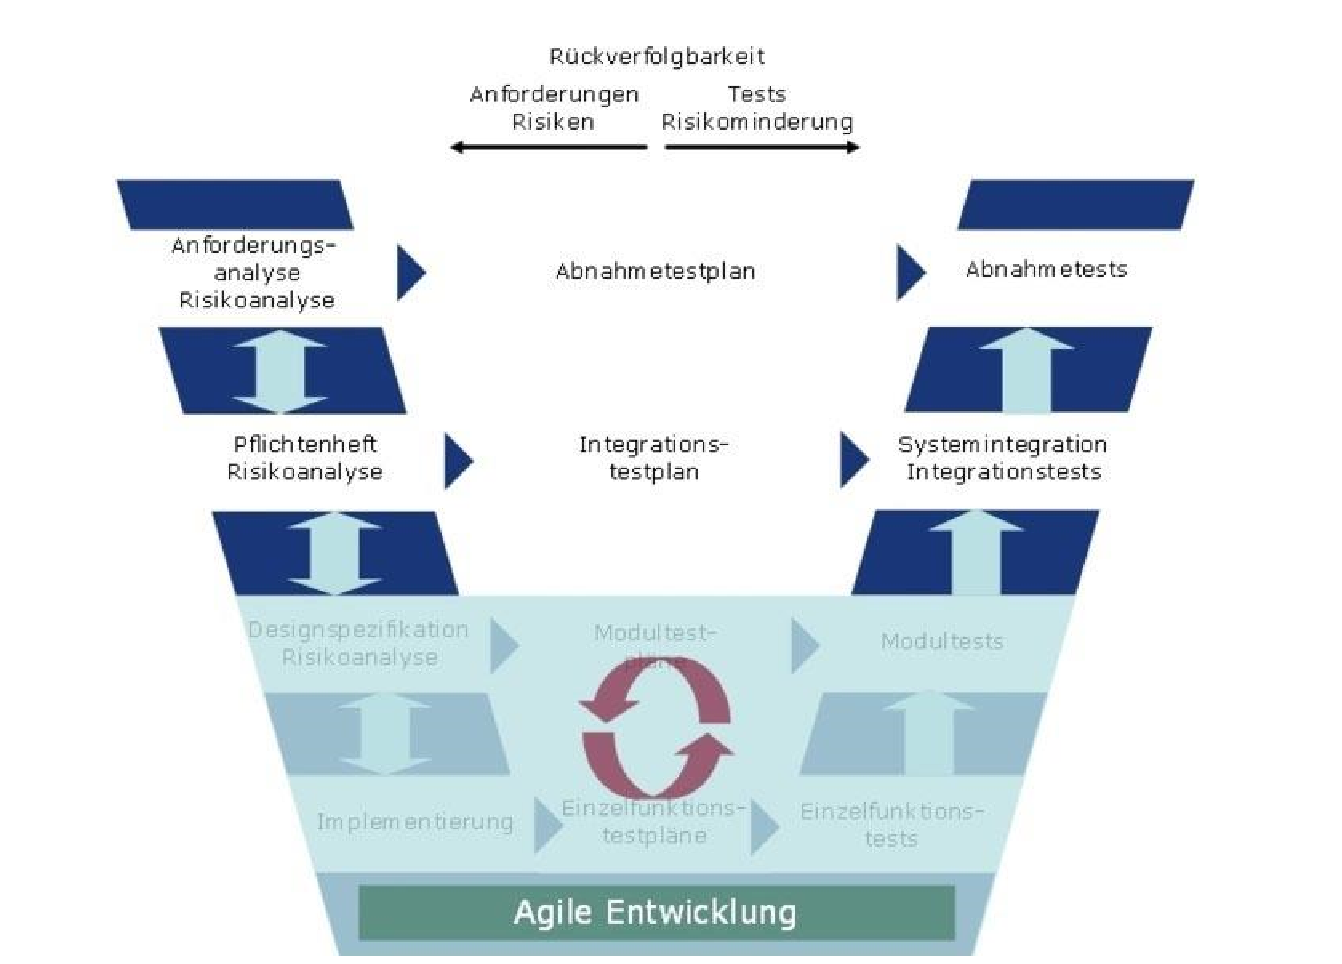
\includegraphics[width=0.89\textwidth]{hybridesModell}
		\caption[Hybrides Vorgehensmodell]{Hybrides Vorgehensmodell \\ (Quelle: https://www.eckelmann.de/en/services/development-process-models)}
		\label{fig:hybridesModell}
	\end{center}
\end{figure}


\subsection{Zeitplanung}
\label{sec:zeitplanung}
Die folgenden Abbildungen stellen die Projektplanung und die Meilensteine zeitlich dar (\seeref{fig:projektPlanungAchse} \& \cref{fig:projektPlanung}). In die erste Woche werden die Hardwarekomponenten, die mittlerweile schon bestellt wurden, getestet und zusammengebaut. 
\\
Die nächste zwei Hauptpunkte betreffen die Programmierung der  Software, die in zwei Teile geteilt wurde.
\\ 
Beim Teil 1 geht es um die Skripts die serverseitig kleine Aufgaben übernehmen, beim Teil 2 geht es um die Programmierung der Software. Da werden die Webapplikationen entwickelt, die auf den Aussensprechstellen und auf den mobilen Geräten der Bewohner ausgeführt werden sollen.
\\
Die letzte Phase ist für die Optimierung und als Reserve gedacht.

\begin{figure}[htb!]
	\begin{center}
		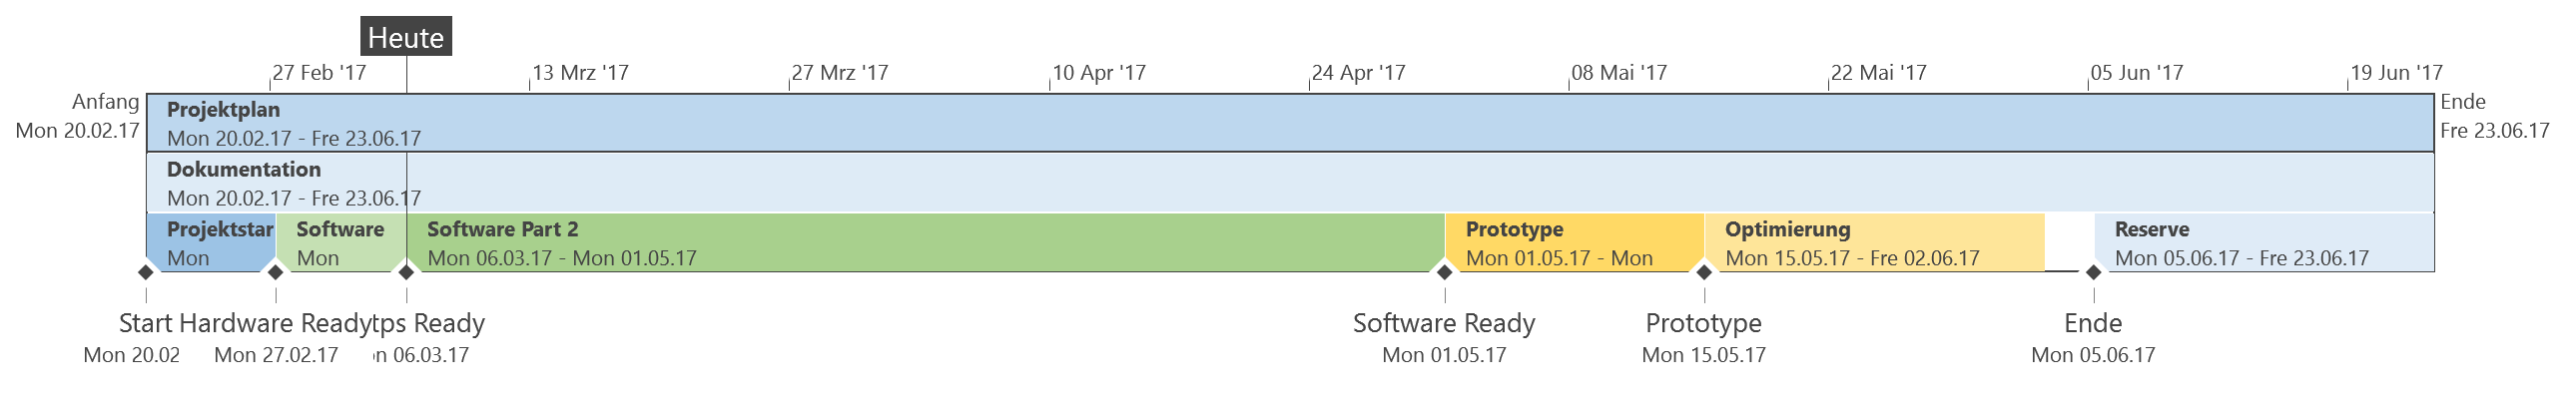
\includegraphics[width=1\textwidth]{projektPlanAchse}
		\caption[Projektplanung Meilensteine]{Zeitplanung mit Meilensteine}
		\label{fig:projektPlanungAchse}
	\end{center}
\end{figure}


\begin{figure}[htb!]
	\begin{center}
		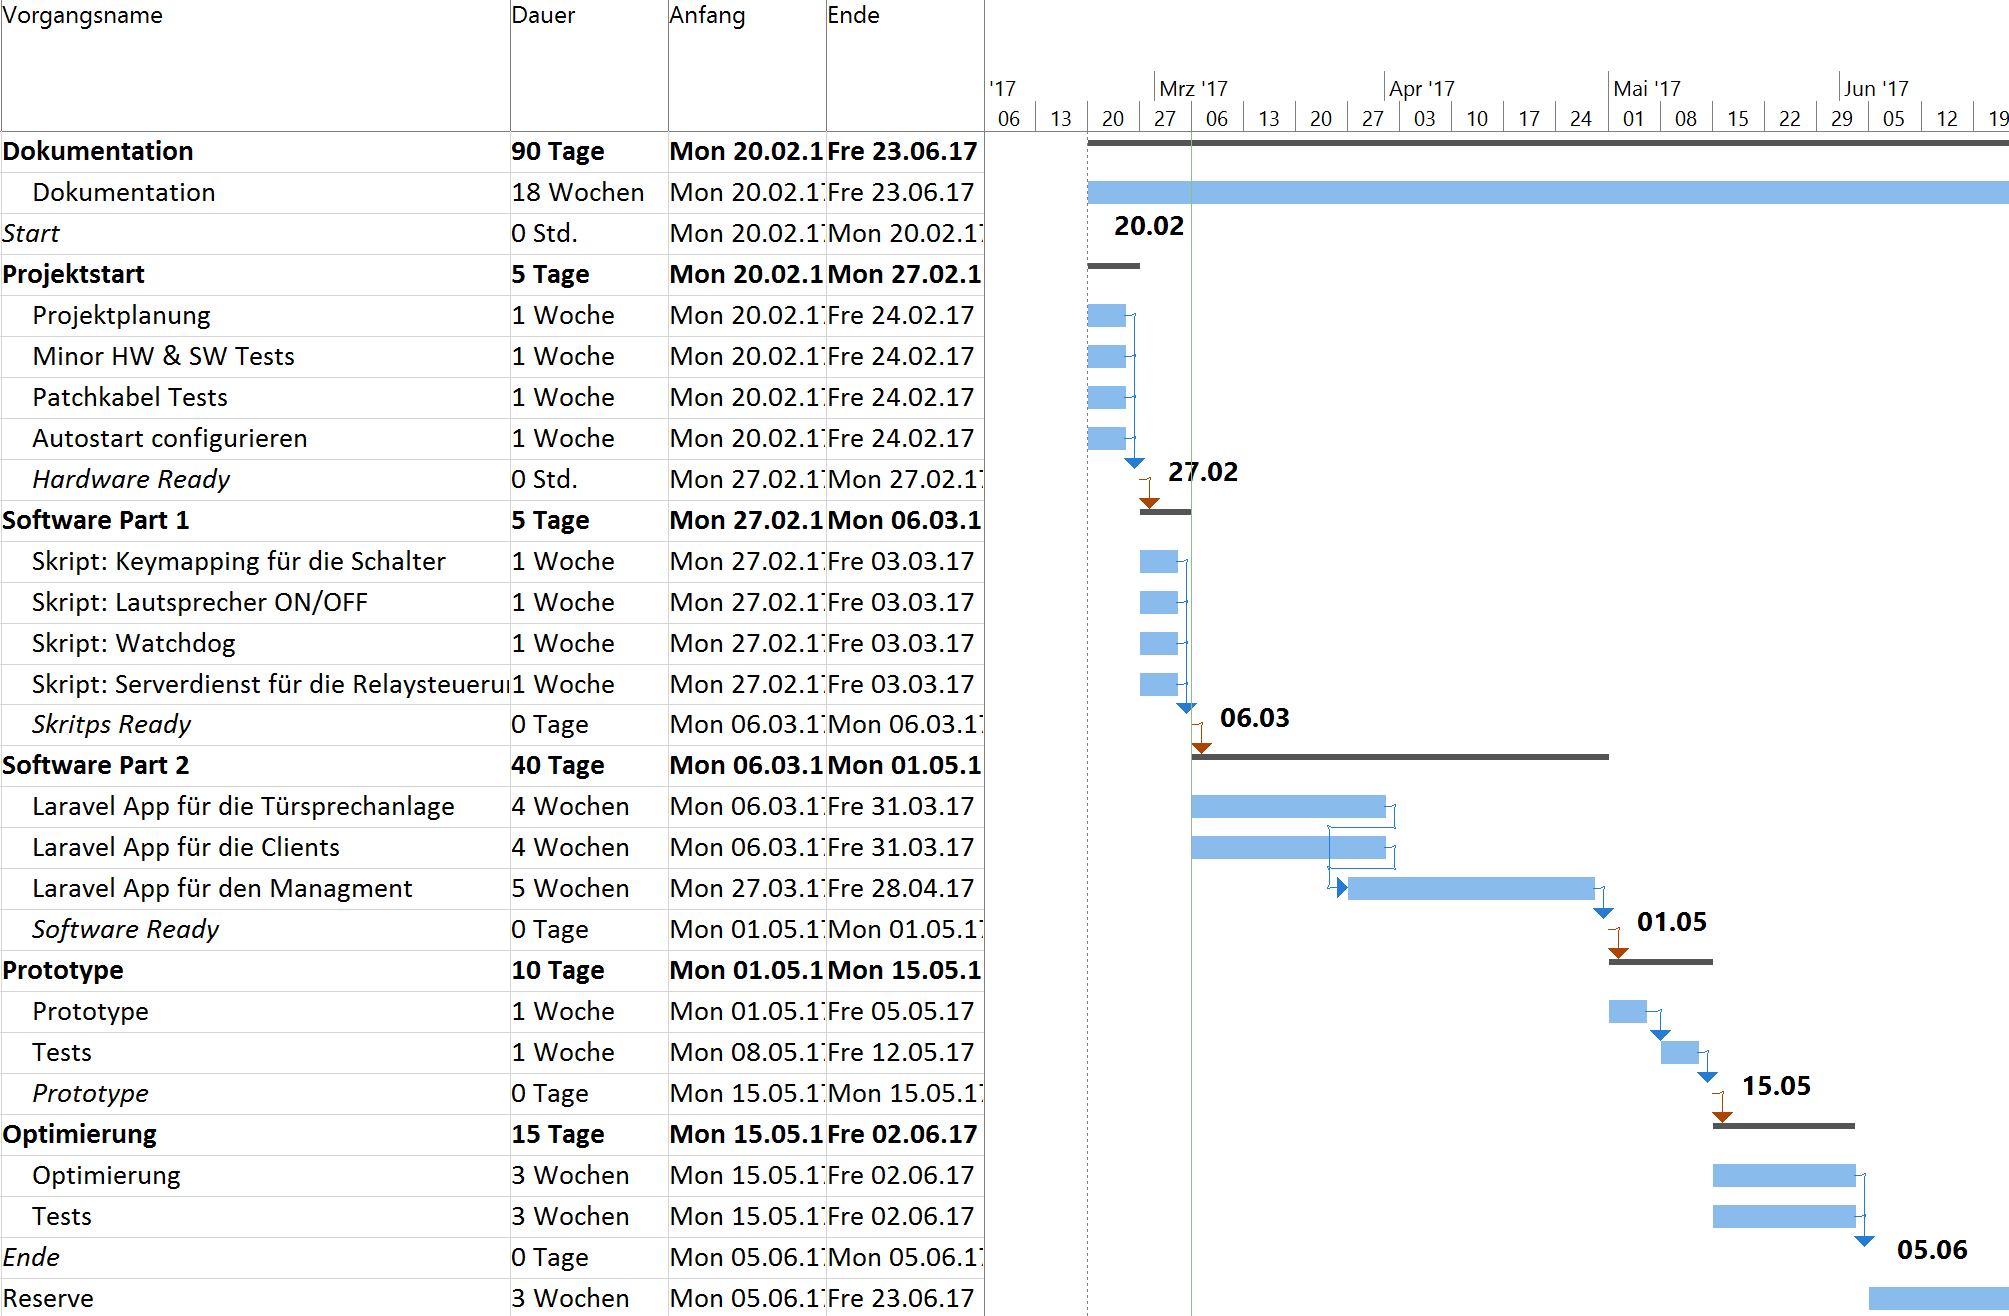
\includegraphics[width=0.9\textwidth]{projektPlanung}
		\caption[Projektplanung]{Projektplanung}
		\label{fig:projektPlanung}
	\end{center}
\end{figure}

\subsection{Versionierung}
Für die Versionierung und die gesamte Entwicklung wird das etablierte Open-Source Version-Control Software GIT verwendet. Das gesamte Quellcode, alle Bilder und Dokuemente werden in einem Repository gespeichert und versioniert.
\\
\\
Während die Entwicklung wird der Quellcode aber nicht Open-Source sein. Das Quellcode und die gesamte Entwicklungsdokumentation für das Projekt wird Vertraulich gehalten und nur für die Entwickler und Projektteilnehmer verfügbar sein. Für die Repository und das Backup wird also den Consumer Dienst Bitbucket verwendet.
\\
\\
Bitbucket (\seeref{fig:bitbucket}) ist ein webbasierter Filehosting-Dienst für Software-Entwicklungsprojekte, der die Versionsverwaltungssysteme Git und Mercurial unterstüzt. Bitbucket ermöglicht auch die Zusammenarbeit von mehreren Benutzern am gleichen Projekt. Bitbucket ist für ein Projekt dieser grosse kostenfrei.
\begin{figure}[htb!]
	\begin{center}
		
\includegraphics[width=1\textwidth]{bitbucket}
		\caption[Bitbucket ist ein Filehosting und ein Dienst für die Versionskontrolle von Softwareprojekte]{Bitbucket ist ein Filehosting und ein Dienst für die Versionskontrolle von Softwareprojekte}
		\label{fig:bitbucket}
	\end{center}
\end{figure}

\subsection{Risikoanalyse}
Inhalt der Risikoanalyse ist die frühzeitige Identifikation, das Bewerten von Problemen und das Definieren von Massnahmen die zu der Risikominimierung führen.
\\
Der Risiko-Management Prozess nach ISO 31000:2009 umfasst folgende Hauptpunkte: 

\begin{itemize}
	\item Risikoidentifikation: Liefert eine Liste von möglichen Risiken die während der Implementierungsphase auftreten könnten. 
	\item Aufgrund der Risikoidentifikation werden Zusammenhänge zwischen den Risiken und die Auswirkungen auf dem Projekt beurteilt. 
	\item Risikobewertung: Zu jedem Risiko werden die Eintrittswahrscheinlichkeit sowie die Auswirkung auf das Gesamtprojekt abgeschätzt.
	\item Risikobewertung: Zu jedem Risiko werden die Eintrittswahrscheinlichkeit sowie die Auswirkung auf das Gesamtprojekt abgeschätzt.
	\item Risikosteuerung: Maßnahmen planen, um die gemessenen und analysierten Risiken zu steuern.
\end{itemize}

\subsubsection{Identifikation Analyse und Bewertung}
Die Identifikation der Risiken erfolgte durch Brainstorming, aber auch durch Probleme die während den Sitzungen und der Projektplanerfassung aufgetaucht sind.
\\
\\
Um die aufgelisteten Risiken zu bewerten, wurde eine Risikomatrix eingesetzt. Diese soll eine visuelle Darstellung von Risikobewertungen geben. 
\begin{figure}[htb!]
	\begin{center}
		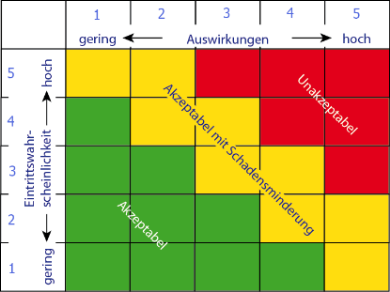
\includegraphics[width=0.5\textwidth]{risikomatrix}
		\caption[Risikomatrix]{Risikomatrix}
		\label{fig:risikomatrix}
	\end{center}
\end{figure}
\\
Die Auswirkungen sowie die Eintrittswahrscheinlichkeit werden mit einem Index (0 bis 5) von gering bis hoch eingestuft. Das Risiko ergibt sich durch die Multiplikation der beiden Achsen. Die Risiken die sich im roten Bereich der Matrix befinden, müssen bei der Risikosteuerung/Maßnahmen sehr intensiv und detailliert behandelt werden, damit einer der beiden Faktoren minimiert werden kann. 
\\
\subsubsection{Bewertung Projekt Risiken}
Die folgende Tabellen stammen aus dem Fachmodul.
\begin{figure}[htb!]
	\begin{center}
		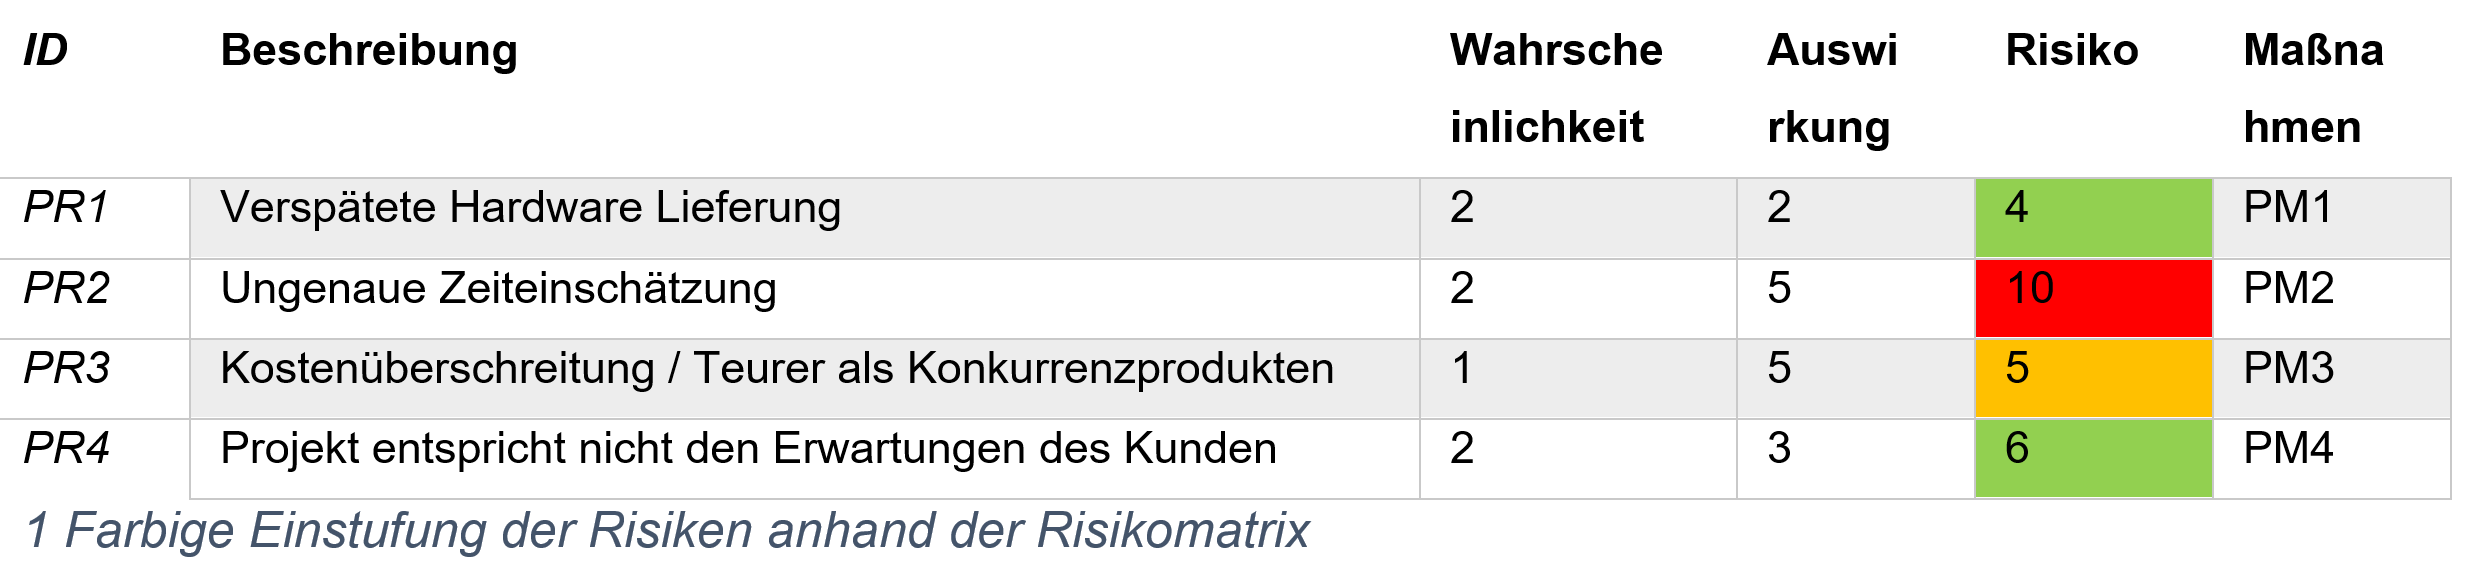
\includegraphics[width=0.95\textwidth]{projektrisiken}
		\caption[Bewertung Projekt Risiken]{Bewertung Projekt Risiken}
		\label{fig:projektrisiken}
	\end{center}
\end{figure}
\subsection{Bewertung Technische Risiken}
\begin{figure}[htb!]
	\begin{center}
		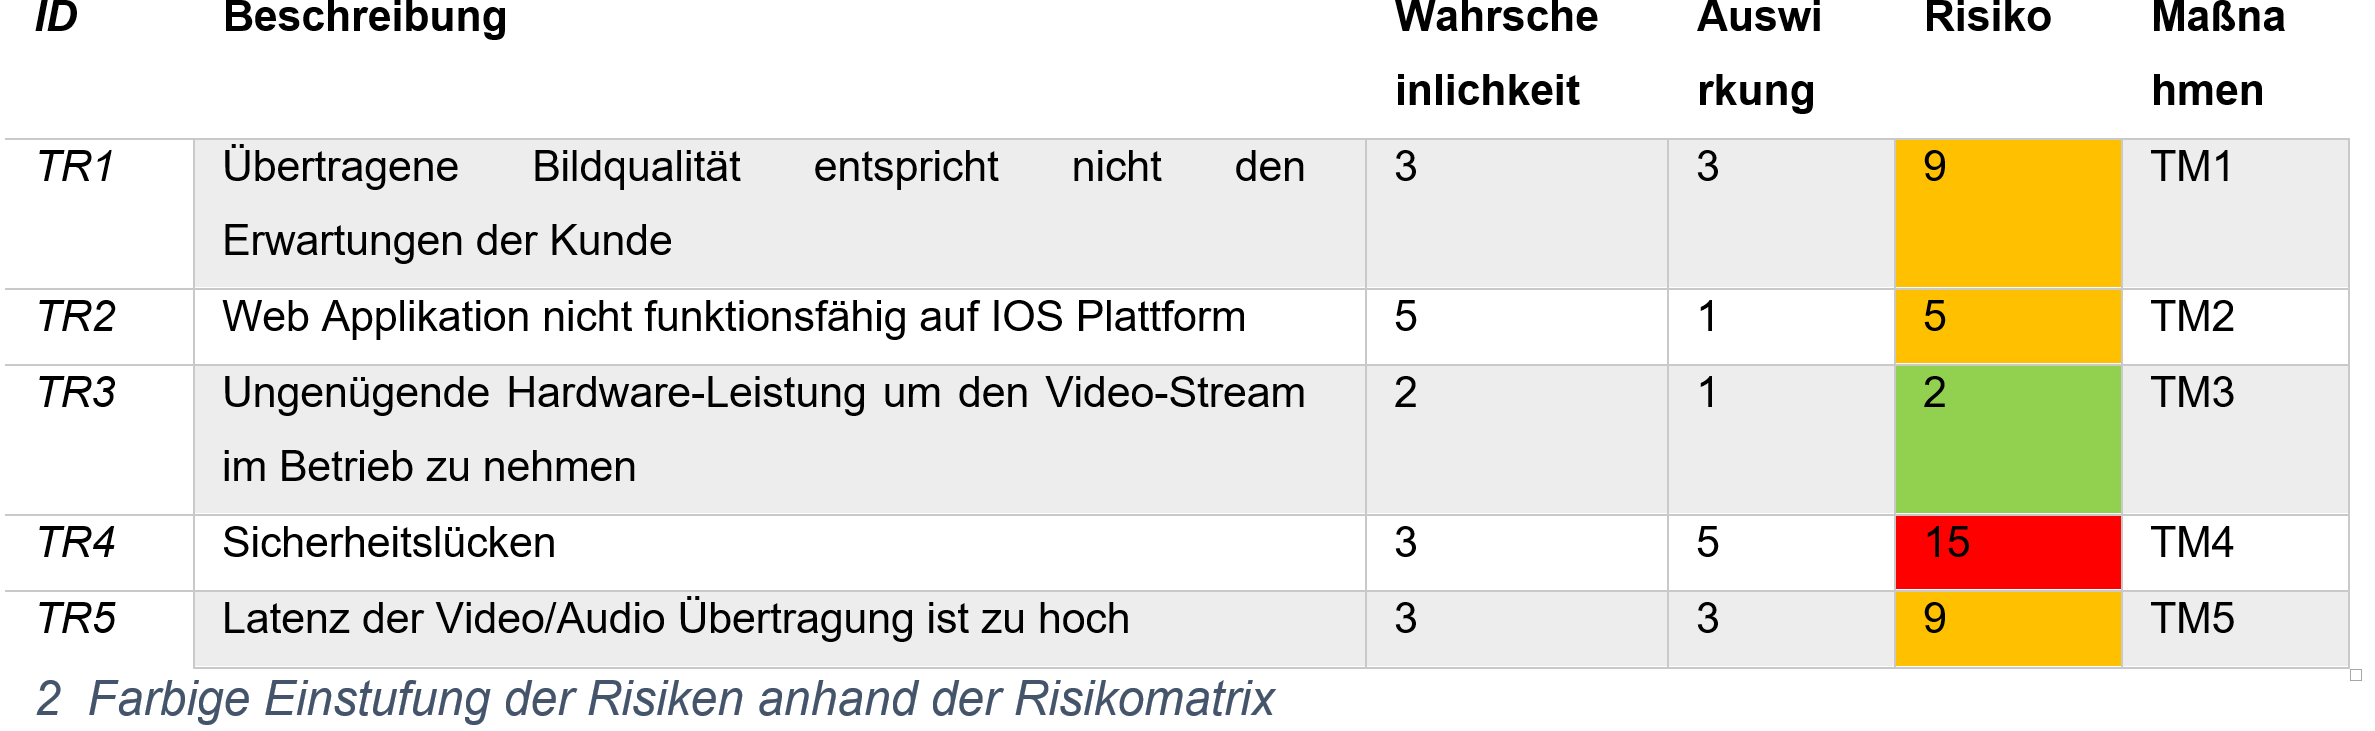
\includegraphics[width=0.9\textwidth]{bewertungrisiko}
		\caption[Bewertung Technische Risiken]{Bewertung Technische Risiken}
		\label{fig:techrisiko}
	\end{center}
\end{figure}
\subsubsection{Risikosteuerung \& Projekt Massnahmen}
\begin{figure}[htb!]
	\begin{center}
		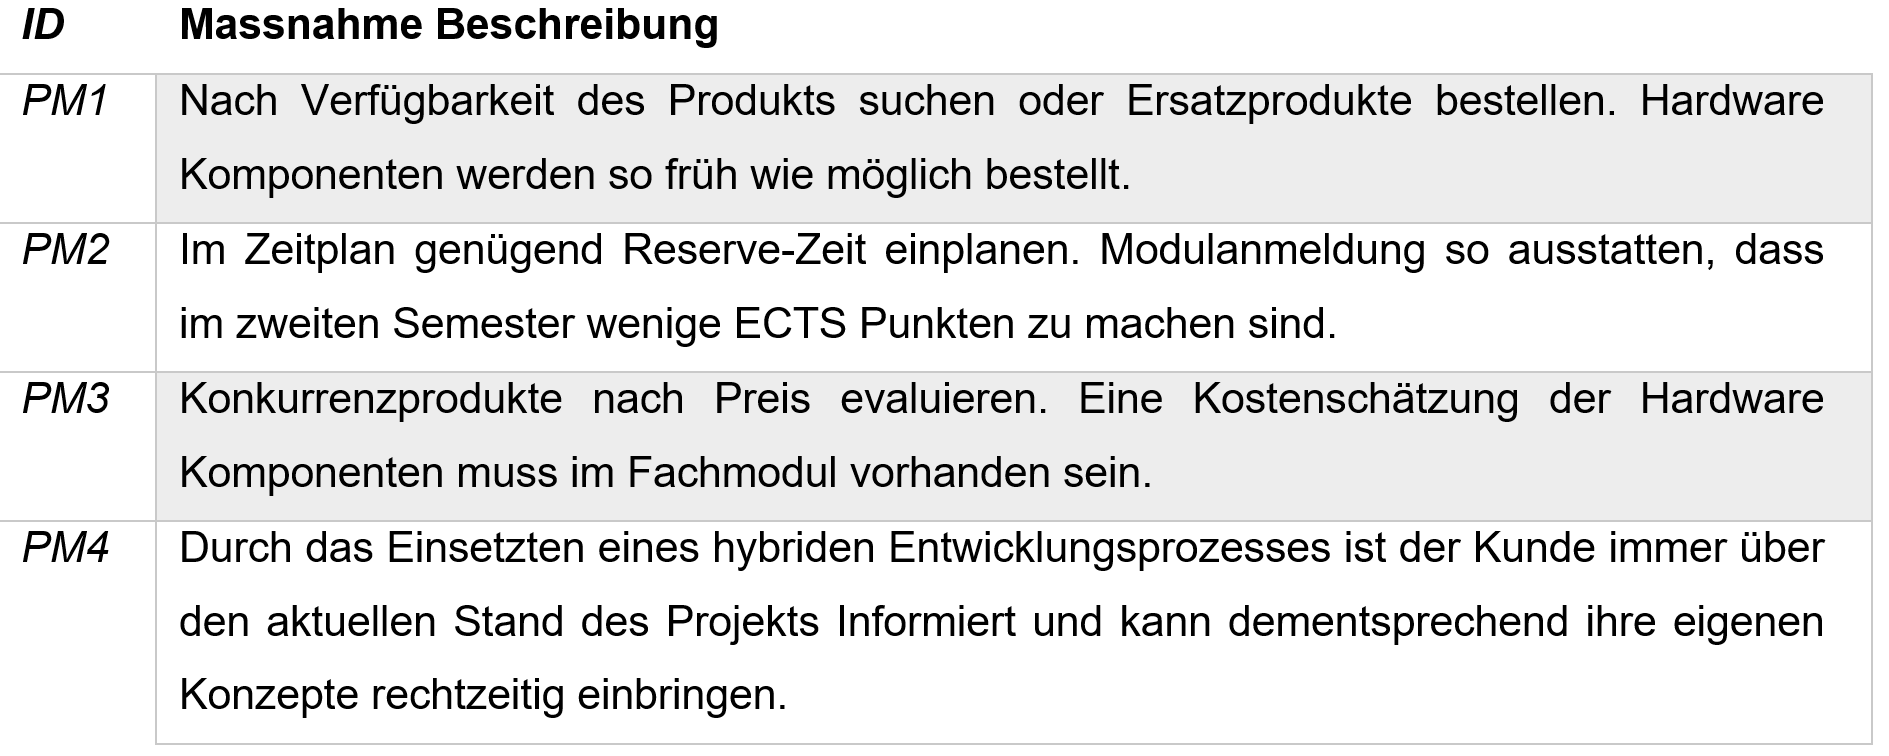
\includegraphics[width=0.75\textwidth]{massnahmen}
		\caption[Projekt Massnahmen]{Projekt Massnahmen}
		\label{fig:risikomassnahmen}
	\end{center}
\end{figure}

\newpage

\section{Aktueller Stand}
\label{sec:chapterexample}

Eine Türsprechanlage, welche Audio und Video überträgt ist keine neue Erfindung. Auf dem Markt existieren bereits verschiedene Lösungen und das schon seit mehreren Jahren. Diese sind aber meistens Analoge Systeme und verfügen über die Vorteile der Digitalisierung nicht. Die Steuerung über eine Mobileapplikation ist bei solche Lösungen aus diesem Grund ausgeschlossen.

\begin{figure}[htb!]
	\begin{center}
		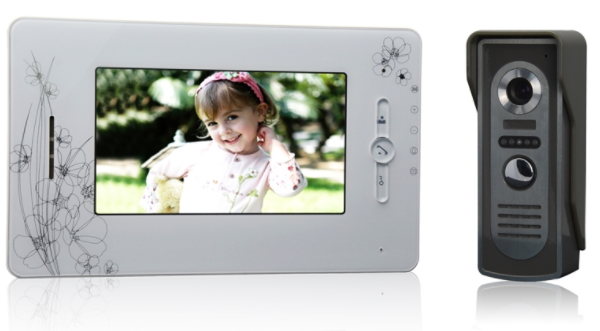
\includegraphics[width=0.66\textwidth]{analog_intercom}
		\caption[Analoge Türsprechanlage mit In-House Display]{Analoge Türsprechanlage mit In-House Display}
		\label{fig:analoge_intercom}
	\end{center}
\end{figure}

In den letzten Jahren sind die ersten Digitale Lösungen mit IP Videoübertragung auf dem Markt gekommen. Die Digitalisierung in diesem Bereich hat es die gigantische Schritten im Bereich der Miniaturisierung und die immer schnellere Internet Zugänge (xDSL, LTE, usw) zu verdanken.

\subsection{Die Herausforderungen der Digitalisierung}
Die Digitalisierung bringt nicht nur Vorteile mit sich. Besonders bei der Video und Audioübertragung. Während eine Analoge Videoübertragung ziemlich mühelos erfolgt muss im Fall eine Digitale Lösung das Video zuerst kodiert und dann dekodiert werden.
\\
Die heutige Kodierung-Algorithmen ermöglichen eine ziemlich schnelle Dekodierung. Mittlerweile hat jeder Smartphone genug Leistung um ein Full-HD Videostream vom Youtube oder Netflix in real-time zu dekodieren. Auf die andere Seite ist die Kodierung ein sehr rechenintensiven Prozess und benötigt sehr viel Leistung.
\\
Jeder der schon mal mit Video-Editing zu tun hatte, weisst, wie viel Zeit die Exportierung eines Video dauern kann.
\\
Die grösste Herausforderung für die real-time Digitale Video/Audio Kommunikation besteht also darin, die Kodierung und Dekodierung der Audio und Video Signal im vernünftigen Zeit durchzuführen. 

\subsection{Marktsituation}
\label{sec:chapterexample}
Der Hauptziel dieses Bachelorarbeit ist, eine Kostengünstige Lösung für eine digitale, flexible und skalierbare Gegensprechanlage. Tatsächlich ist es so, dass die bestehende Lösungen sehr teuer sind. Viele Produkte basieren auf Drittanbieter, SIP Gateways oder andere Elemente die Zusatzkosten verursachen. Das möchten wir alles vermeiden.

\begin{figure}[htb!]
	\begin{center}
		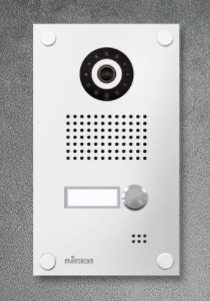
\includegraphics[width=0.33\textwidth]{myintercom}
		\caption[Telecom Behnkle MyIntercom]{Telecom Behnkle MyIntercom}
		\label{fig:myintercom}
	\end{center}
\end{figure}

Eine der günstigsten Produkte den wir finden konnten ist das \textit{"MyIntercom"} von Telecom Behnkle (\seeref{fig:myintercom}). Diese Türklingelanlage ist ziemlich flexibel und bietet die Möglichkeit, mehrere Türen anzuschliessen. Der Preis liegt hier bei zirka 1'600.- CHF pro Türe bei dem Basic-Modell.
\\
\\
 Dank der Aufschwung von Open-Source Hardware wie das Raspberry PI und Real Time Communication Protokolle wie WebRTC muss es möglich sein, kostengünstigere Lösungen zu erarbeiten. Bei den folgenden Kapiteln geht es nun um die effektive Realisierung einem Prototyp, welches die oben genannte Problemen adressiert. 

\newpage
\section{Anforderungen}
Für den Bachelorarbeit wurden die Anforderungen bereits in dem Fachmodul definiert.
\subsection{Anforderungen}
A1. Es soll möglich sein, die Haustüre durch ein Signal zu öffnen. 
\\
\\
A2. Es soll möglich sein, ein Videosignal von der Aussensprechstelle zum Client zu streamen. 
\\
\\
A3. Es soll möglich sein, ein Audiosignal zwischen der Aussensprechstelle und der Client App bidirektional zu streamen. 
\\
\\
A4. Ein digitaler Bildschirm zeigt die Informationen der Bewohner (Name, Vorname, usw) an der Aussensprechstelle an. 
\\
\\
A5. Nach einem Stromunterbruch soll die Anlage automatisch wieder Starten und Funktionsbereit sein. 
\\
\\
A6. Den Datenverkehr zwischen den Endknoten muss Verschlüsselt sein. 
\\
\\
A7. Die Komponenten sollten zwischen -20C und +40C funktionsfähig sein. 
\\
\\
A8. Die Komponenten sollten auch im Fall hoher Feuchtigkeit funktionsfähig sein. (80\%) 
\\
\\
A9. Die Kamera für das Videosignal muss eine Auflösung von mind. 1280x720 Pixel aufweisen.  
\\
\\
A10. Die Materialkosten pro Aussensprechstelle sollten 400.- nicht überschreiten. 
\\
\\
A11. Die Aussensprechstelle soll auch mit nasse/bedeckte Hände bedienbar sein. 
\\
\\
A12. Bei der Innenstelle ist es möglich das Mikrofon auszuschalten, um die Übertragung des Audiosignales zu unterdrücken. 

\subsection{Wunschanforderungen}
W1. Die Komponenten sollten die Speisung durch PoE erhalten. 
\\
\\
W2. Die Kamera für das Videosignal muss eine Auflösung von 1920x1080 Pixel aufweisen. 
\\
\\
W3. Verpasste Besuche sollten aufgezeichnet werden und in der Client App in Form von einem Foto und Notifikation sichtbar sein.
\newpage

\section{Lösungskonzept}
\label{sec:lösungskonzept}
Die \cref{fig:hwoverview} zeigt einen Überblick über die verschiedenen Hardwarekomponenten, die für die \gls{turklingelanlage} benötigt werden.
\\
Es werden nun zwei Begriffe erklärt, die in diesem Dokument von grosse Bedeutung sind. Das erste ist die \gls{turklingelanlage}. Damit gemeint ist die Gesamtheit der Komponenten die denn Zusammen den Endprodukt darstellen.
\\
Als \gls{aussensprechstelle} ist die Gesamtheit aller Komponenten des Endproduktes gemeint, als Aussensprechstelle der an der Eingangstüre installierte Mikrocontroller inklusive dazugehörige Module.
\\
Räumlich von der \gls{aussensprechstelle} getrennt befindet sich der Server. Dieser besteht aus einem Mikrocontroller, der als Server im Einsatz steht, aus einem Switch der dazu dient die \gls{aussensprechstelle} mit Strom und Datenverbindung zu versorgen und aus einem Relais welches den Türöffner und die Glocke betätigt.
\begin{figure}[htb!]
	\begin{center}
		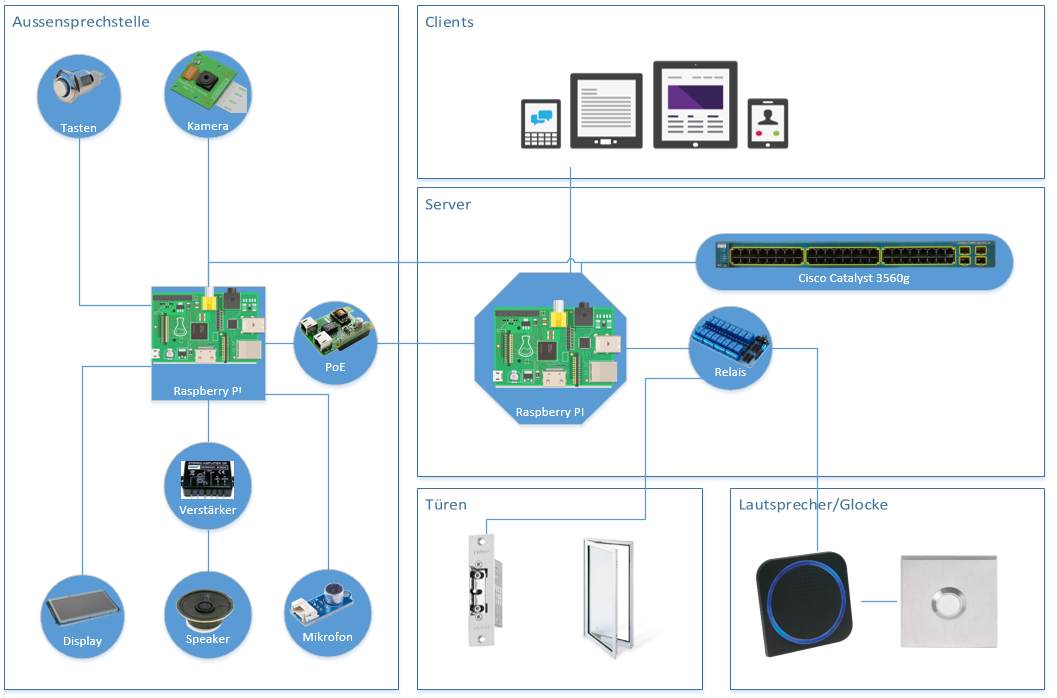
\includegraphics[width=0.95\textwidth]{hwoverview}
		\caption[Hardware Ecosystem]{Hardware Ecosystem}
		\label{fig:hwoverview}
	\end{center}
\end{figure}
Das System besteht aber nicht nur aus Hardware. Das Zusammenarbeiten der Hardware wird von viel Softwareelemente geregelt. Als erstes, wie bereits in der Projektplanung definiert, wird die Hardwareseite der Lösung realisiert. Sobald alle Hardwarekomponenten getestet und auf Kompatibilität geprüft worden sind, wird die Programmierung stattfinden.
\newpage

\section{Umsetzung der Hardware}
\label{sec:chapterexample}
\subsection{Komponenten}
Das System wird hardwareseitig grob in zwei Teile unterteilt, den Server und die \gls{aussensprechstelle}.
\\
Die \cref{tbl:SrvHW} und die \cref{tbl:DoorHW} zeigen die benötigten Hardwarekomponenten, welchen an den jeweiligen Stellen eingebaut werden.
\\
Um den Überblick über die Kosten aller Hardwarekomponenten zu behalten, sind hier auch die Preisen aufgelistet. Dabei ist es wichtig sicherzustellen, dass die gesamten Hardwarekosten diejenigen der von der Konkurrenz angebotenen Produkte nicht übersteigen.
\\
Die Einkaufspreise sind nur Richtpreise, da es sich um Standardkomponenten handelt und die Marktpreise sich ständig und schnell ändern können. Die Summen sind als Kostenschätzung zu betrachten. (Stand Fruhjahr 2017).

\begin{table}[]
	\centering
	\label{my-label}
	\begin{tabular}{l|ll}
		\multicolumn{1}{r|}{} \textbf{Anzahl} & \textbf{Komponente} \hspace{180pt} & \textbf{Preis} 	\\ \hline
		1	&	Raspberry Pi 3 Model B						& 50.-				\\ \hline
		1	&	Raspberry Gehäuse und Netzteil				& 25.-			\\ \hline
		2	&	8-Kanal Relais Modul						& 15.-			\\ \hline
		1	&	\textit{Kleinmaterial}						& 15.-			\\ \hline
		\textbf{Total}	&									& \textbf{140.-}			\\ \hline
	\end{tabular}
	\caption{Server \gls{hw} Komponenten}
	\label{tbl:SrvHW}
\end{table}

\begin{table}[]
	\centering
	\label{my-label}
	\begin{tabular}{l|ll}
		\multicolumn{1}{r|}{} \textbf{Anzahl} & \textbf{Komponente} \hspace{180pt} & \textbf{Preis} 	\\ \hline
		1	&	Raspberry Pi 3 Model B		   				& 50.-			\\ \hline
		1	&	4" Bildschirm								& 64.-			\\ \hline
		1	&	Raspberry Kamera							& 59.-			\\ \hline
		1	&	\gls{poe} Adapter									& 50.-			\\ \hline
		3	&	Schalter									& 25.-			\\ \hline
		1	&	Mikrophon									& 12.-			\\ \hline
		1	&	Lautsprecher								& 9.-			\\ \hline
		1	&	Audio Verstärker							& 10.-			\\ \hline
		1	&	\textit{Kleinmaterial / Gehäuse}			& 50.-			\\ \hline
		\textbf{Total}	&									& \textbf{329.-}			\\ \hline
	\end{tabular}
	\caption{Aussensprechstelle \gls{hw} Komponenten}
	\label{tbl:DoorHW}
\end{table}

\subsection{Stromspeisung}
\label{sec:poe}
Ein Ziel unserer Lösung ist die Installationskosten zu senken und die Montage zu vereinfachen. Aus diesem Grund war für unsere Lösung wichtig, \gls{poe} zu verwenden. In modernen Haushalte werden meistens Ethernet Verkabelungen verlegt und dank PoE ist nur noch ein Kabel, welches Strom und Konnektivität gewährleistet, notwendig.
\\
\\
Zusätzlich benötigt das System noch eine Leitung die den Türöffner steuert.
Auch diese Endinstallation kann vereinfacht werden wenn man, anstatt ein dediziertes Kabel zwischen Server und Türöffner einzuziehen,  zwei Drähte des bereits installierten Ethernet Kabels verwendet.
\\
\\
Cisco Catalyst 3560g welcher für den \gls{poe} Stromversorgung zuständig ist, verwendet die Phantomspeisung oder Mode A. Das heisst, dass die mit der Datenübertragung belegten Drähte mit der Stromversorgung überlagert werden. Dies ist möglich da die Frequenz der Elektrizität 60 Hz beträgt und die der Datenübertragungen im Bereich von 10-100MHz liegt.

\begin{figure}[htb!]
	\begin{center}
		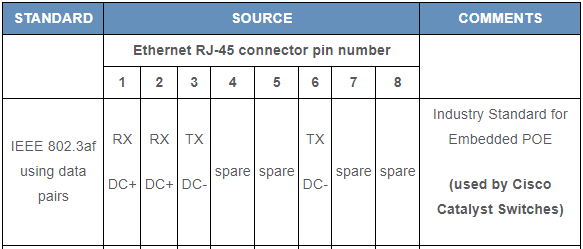
\includegraphics[width=0.89\textwidth]{CatalystPoEpinouts}
		\caption[Catalyst Pinouts]{Catalyst 3560g \gls{poe} Pinbelegung}
		\label{fig:catalystPinouts}
	\end{center}
\end{figure}

Wie im \cref{fig:ethernetBelegung} dargestellt werden die Adern 7 und 8 dazu verwendet um den Türöffner zu betätigen. Aus den 3 verbliebenden Adernpaaren kann maximal die Ethernetkategorie 100BASE-T erreicht werden. Da aber \gls{webrtc} eine erhebliche kleinere Bandbreite in Anspruch nimmt, stellt es für die \gls{aussensprechstelle} kein Hindernis dar.

\begin{figure}[htb!]
	\begin{center}
		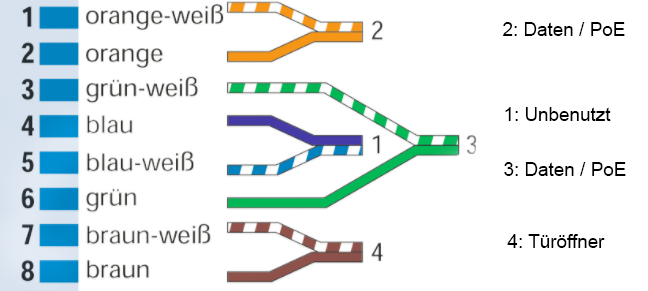
\includegraphics[width=0.89\textwidth]{EthernetPinbelegung}
		\caption[EthernetPinbelegung]{Cat. 7 Ethernet Pinbelegung der \gls{aussensprechstelle}}
		\label{fig:ethernetBelegung}
	\end{center}
\end{figure}



\subsection{Server}
\label{sec:chapterexample}
Der Server wird mit einem Relais-Board verbunden um die Gongs und die Türöffner zu bedienen. An dieser Stelle ist die Hardwarekonfiguration sehr einfach. Mit der aktuellen Hardwarekonfiguration könnten bis 8 Wohnungen und 8 Aussensprechstellen angeschlossen werden. Die \cref{fig:pipins} und die \cref{fig:boardpins} zeigen die Pinbelegung auf dem Pi und auf dem Relais-Board. Die \cref{tbl:pinroutes} zeigt wie die verschiedenen Pins miteinander verbunden werden.

\begin{figure}[htb!]
	\begin{center}
		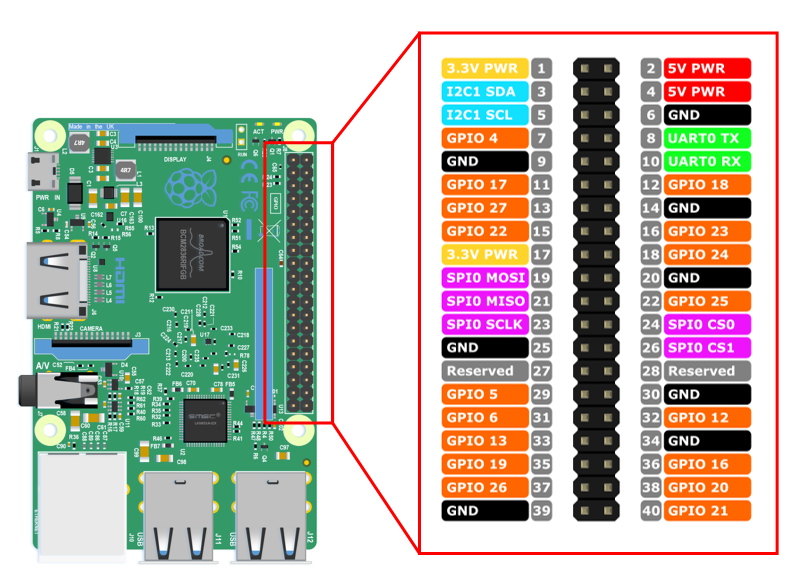
\includegraphics[width=0.8\textwidth]{pipins}
		\caption[EthernetPinbelegung]{Pinbelegung der \gls{aussensprechstelle}}
		\label{fig:pipins}
	\end{center}
\end{figure}

\begin{figure}[htb!]
	\begin{center}
		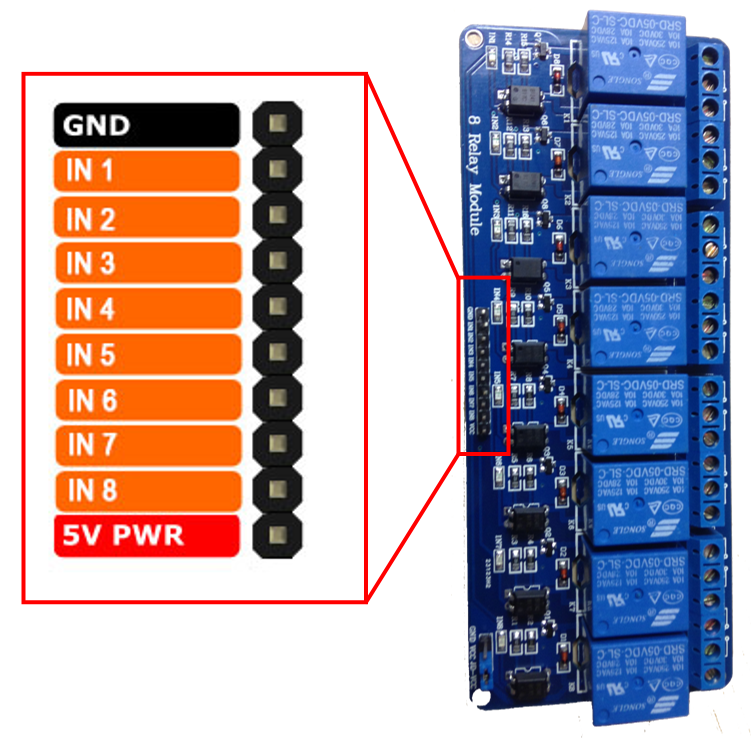
\includegraphics[width=0.55\textwidth]{boardpins}
		\caption[EthernetPinbelegung]{Pinbelegung für das Relais-Modul}
		\label{fig:boardpins}
	\end{center}
\end{figure}

\begin{table}[]
	\centering
	\label{my-label}
	\begin{tabular}{l|ll}
		\multicolumn{1}{r|}{} \textbf{Pi GPIO (PIN)} & \textbf{Relais IN (Board Nr)} & \textbf{Funktion}  \hspace{60pt}	\\ \hline
		GPIO4 (7)	&	IN1 (1)			& Gong WG.1			\\ \hline
		GPIO17 (11)	&	IN2 (1)			& Gong WG.2			\\ \hline
		GPIO27 (13)	&	IN3 (1)			& Gong WG.3			\\ \hline
		GPIO22 (15)	&	IN4 (1)			& Gong WG.4			\\ \hline
		GPIO5 (29)	&	IN5 (1)			& Gong WG.5			\\ \hline
		GPIO6 (31)	&	IN6 (1)			& Gong WG.6			\\ \hline
		GPIO13 (33)	&	IN7 (1)			& Gong WG.7			\\ \hline
		GPIO19 (35)	&	IN8 (1)			& Gong WG.8			\\ \hline
		GPIO18 (12)	&	IN1 (2)			& Türöffner Türe 1			\\ \hline
		GPIO23 (16)	&	IN2 (2)			& Türöffner Türe 2			\\ \hline
		GPIO24 (18)	&	IN3 (2)			& Türöffner Türe 3			\\ \hline
		GPIO25 (22)	&	IN4 (2)			& Türöffner Türe 4			\\ \hline
		GPIO12 (32)	&	IN5 (2)			& Türöffner Türe 5			\\ \hline
		GPIO16 (36)	&	IN6 (2)			& Türöffner Türe 6			\\ \hline
		GPIO20 (38)	&	IN7 (2)			& Türöffner Türe 7			\\ \hline
		GPIO21 (40)	&	IN8 (2)			& Türöffner Türe 8			\\ \hline
	\end{tabular}
	\caption{PIN-Zuweisung zwischen den Server und die Relais Module}
	\label{tbl:pinroutes}
\end{table}


\subsection{Aussensprechstelle}
\label{sec:chapterexample}
Bei der \gls{aussensprechstelle} wird auch ein Raspberry Pi eingesetzt. Hier sind mehrere Zusatzkomponenten notwendig. Die Speisung, wie oben schon erwähnt, erfolgt an dieser Stelle über \gls{poe}. Aus diesem Grund ist ein \gls{poe}-Splitter vorhanden.
\\
Für die Audiowiedergabe sind ein kleiner Lautsprecher und ein Verstärker notwendig. Der Chinch Anschluss des Raspberrys Pi hat eine zu niedrige Ausgangsleistung um den Lautsprecher direkt anschliessen zu können.
\\
Die drei Schalter, die für die Bedienung der \gls{aussensprechstelle} notwendig sind, werden an die \gls{gpio}s des Raspberrys PI angeschlossen. Die \cref{tbl:pinroutesdoor} zeigt die Pinbelegung.

\begin{table}[]
	\centering
	\label{my-label}
	\begin{tabular}{l|ll}
		\multicolumn{1}{r|}{} \textbf{Pi GPIO (PIN)} & \textbf{Schalter} & \textbf{Funktion} \hspace{60pt}	\\ \hline
		GPIO16 (36)	&	Schalter Links		&	Nach Links Scrollen	\\ \hline
		GPIO20 (38)	&	Schalter Mitte		&	Glocke läuten		\\ \hline
		GPIO21 (40)	&	Schalter Rechts		&	Nach Rechts Scrollen		\\ \hline
	\end{tabular}
	\caption{PIN-Zuweisung zwischen den Raspberry PI und die Schalter}
	\label{tbl:pinroutesdoor}
\end{table}

\subsubsection{Problemen}
Während der Zusammenstellung der Aussensprechstelle sind die erste unvorhergesehene Problemen aufgetaucht. Die Audiowiedergabe und Audioaufnahme stellten eine grössere Herausforderung als geplant dar.
\\
\\
\textbf{Audiowidergabe} 
\\
Die grösste Problematik bei der Audiowiedergabe besteht darin, dass die Massen des Raspberrys Pi, des Verstärkers und des Audio-Interface gekoppelt sind. Das führt zu Brummschleifen, die wiederum Störsignale auf dem Audio-Ausgang erzeugen. Um das zu vermeiden, muss an dieser Stelle ein Massentrennfilter eingesetzt werden.
\\
Die Störsignale sind nun fast komplett verschwunden, nur ein winziges Hintergrundgeräusch ist immer noch vorhanden. Um dieses Problem umzugehen, wird ein zusätzliches Relais installiert, welches den Lautsprecherstromkreis bei Nichtnutzung unterbricht.
\\
\\
\textbf{Das Mikrophon}
\\
Das Problem der Audioaufnahme liegt beim Mikrophon selber. Der Raspberry Pi besitzt kein integriertes Audio-Input. Aus diesem Grund wurde ein \gls{usb}-Audio-Interface verwendet. Es hat sich aber herausgestellt, dass es nicht so einfach ist, kostengünstige und qualitatives \gls{usb} Mikrophone zu finden. Die meisten Produkten sind nicht für den Outdoorbetrieb gedacht und oft ist die Empfindlichkeit zu gering um ein qualitatives Audiosignal aufzunehmen.  Für unseren Prototyp wird das eingesetzte Mikrophon völlig ausreichen, für ein gut funktionierendes Endprodukt sollte man ein besseres Mikrophon einbauen.
\newpage
\section{Software}
\label{sec:chapterexample}

\subsection{Programmiersprachen}
Das System besteht aus mehrere Programme und Dienste. Für die Entwicklung werden folgende Programmiersprachen eingesetzt:
\begin{itemize}
	\item Java
	\item Javascript
	\item PHP
\end{itemize}
Im Verbindung mit PHP kommt natürlich die Markup-Languages HTML5/CSS, welche für die graphische Darstellung der Webapplikationen notwendig ist.

\subsubsection{Java}
\label{kap:java}
Alle Dienste die Serverseitig und ohne Interaktion mit dem Enduser ausgeführt werden, werden in Java programmiert. Als stark typisierte und Objektorientierte Programmiersprache eignet sich Java für dieses Projekt. Für Java sind auch unzählige Libraries verfügbar, insbesondere für die Hardware Steuerung der Raspberry Pi. Eine zweite Variante wäre Python gewesen, die auch das Raspberry sehr gut unterstüzt. Python ist aber zu wenig typisiert und für eher kleinere Softwarestücke gedacht.

\subsubsection{PHP/Javascript}
Die Client Applikation sowohl auch die Applikation bei der Aussensprechstelle werden Web-Applikationen sein. Dies ermöglicht eine schnelle und zeitgemässe Softwareentwicklung. Für dieses Projekt ist die System-Eingriffstiefe von Webapplikationen jedenfalls ausreichend. Es muss lediglich Zugriff auf Mikrofon, Lautsprecher und Kamera garantiert werden. Ein weiteres Punkt zugunsten einer Webapplikation ist die Cross-Plattform Kompatibilität.
\\
Aus diesem Grund haben wir uns für PHP (Objektorientiert) im Kombination mit Javascript/HTML/CSS entschieden. Eine zweite Variante wäre Java EE gewesen. Java EE eignet sich aber vor allem für grosse Softwarelösungen und bietet als gesamten Framework vieles mehr als was dieses Projekt benötigt.
\\
\subsubsection{PHP Framework: Laravel}
Für die Entwicklung der Webapplikationen wird Laravel als PHP Framework eingesetzt. Laravel ist ein Open-Source PHP Web-Application-Framework, die sich für kleine bis zu mittelgrosse Projekte eignet. Laravel beruht auf dem Modell-View-Controller-Muster und ermöglicht eine Objektorientierte Programmierung in PHP.

\subsection{System Übersicht}
Das System besteht aus mehrere Hardware- und Softwarekomponenten die zusammenarbeiten müssen (\seeref{fig:echosystem}). Die  Vertraulichkeit der Kommunikation zwischen den Knoten ist von TLS immer gewährleistet. Die einzelne Komponenten, sowie das Thema Sicherheit, werden in den nächsten Kapiteln genauer beschrieben.

\begin{figure}[htb!]
	\begin{center}
		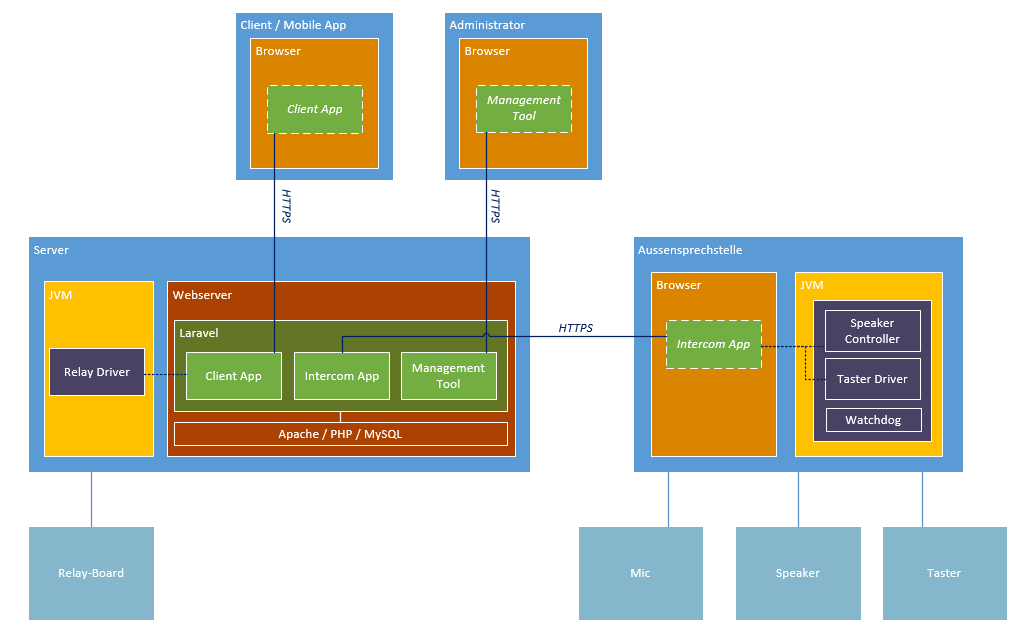
\includegraphics[width=1\textwidth]{ecosystem}
		\caption[Software / Hardware Ecosystem]{Software / Hardware Ecosystem}
		\label{fig:echosystem}
	\end{center}
\end{figure}

Die Software wird in zwei Gruppen unterteilt. Einerseits gibt es alle Dienste/Daemons \textit{(Violett)} die Lokal ausgeführt werden und quasi das Backend des Systems darstellen.
\\
Die zweite Gruppe beinhaltet die Webapplikationen \textit{(Grün)}, die eine GUI besitzen und für die Interaktion mit dem System gedacht sind. Darunter zählen die Client-App für den Bewohner, die Applikation bei der Aussensprechstelle wo die Bewohner angezeigt werden und das Management Tool.
\\
Die Audio/Video-Kommunikation zwischen die Aussensprechstellen und die Client-Apps wird mithilfe von WebRTC realisiert. Diese hat eine gewisse Komplexität und wird in ein eigenes Kapitel (\seeref{kap:webrtc}) behandelt.

\subsection{Raspbian}
\label{kap:raspbian}
Auf alle Raspberry Pi wurde den Betriebssystem Raspbian Jessie installiert. Diese wird von Raspberry Pi Foundation mitgeliefert und gilt als besonders hochoptimerte OS für die mit niedriger Leistung und geringem Stromverbrauch ARM Prozessoren.
Raspbian basiert auf Debian welche unter der DFSG (Debian Free Software Guidelines) Lizent steht. Diese erlaubt der unbeschränkte Weitergabe des Software sowie abgeleitete und modifizierte  Werke weiterzugeben. 
Raspbian enthält Java SE Platform Prudukte welches und dem BCL(Oracle Binary Code License) lizensiert sind. Dieses Lizenz gewährleistet die obengenannten Freiheite ebenfalls.

\subsection{Dienste}
\label{kap:dienste}

\subsubsection{Taster Controller}
Die Aussensprechstelle wird durch 3 Schalter bedient. Die drei Schaltern werden an die GPIO-Pins des Raspberry PI angeschlossen. Die Aufgabe der Taster-Controller besteht darin, die GPIO-Input Signale, als verwendbare Tastatur-Eingaben umzuwandeln. Somit kann die GUI an der Aussensprechstelle gesteuert werden.
\\
Die ursprüngliche Idee war das Taster-Controller, so wie alle andere Dienste, als Daemon auszuführen. Das hätte den Vorteil, dass der Daemon mittels die übliche run, stop und restart Befehle gesteuert werden könnte. Eine der eingesetzten Java-Library benötigt aber den zugriff auf dem Graphisches Umgebung. Das Problem besteht darin, dass ein Daemon Benutzer-Unabhängig ist, während der X-Server beim Login einem Benutzer ausgeführt wird. Das ausführen der Deamon erst ab Init 5, da wo auch der X-Server ausgeführt wird, konnte aus diesem Grund das Problem auch nicht lösen.
Die verwendete Library hat also keine Möglichkeit, als Deamon eine Verbindung mit dem X-Server aufzubauen.
\\\\
Die Desktop-Umgebung LXDE welche von Raspbian verwendet wird, bietet aber ein Autostart welches das Taster-Controller nach dem Initialisierung des X-Server, unter dem gleichen Benutzer ausführt.

\subsubsection{Speaker Controller}
Das Speaker Controller ist ein kleinen Dienst, welche den Lautsprecher ein- und ausschalten kann. Trotz einem Massentrennfilter sind immer noch leise Störsignale auf der Audio-Ausgang vorhanden.
Die Aufgabe des Speaker-Controllers besteht darin, die Stromspeisung des Speakers zu trennen, wenn es nicht verwendet wird. Somit ist das System Energieeffizienter und unnötige Geräusche können vermieden werden.
\\
\\
Der Dienst besteht lediglich aus ein Socket-Server, der auf ein Signal wartet und durch die GPIO der Raspberry, ein kleines Relay steuert.
Das Signal kommt von der Aussensprechstelle-Applikation \textit{(localhost)}. So kann den Lautsprecher bei Bedarf ein- und ausgeschaltet werden.

\subsubsection{Relay Controller}
...
\subsubsection{Signaling Server}
Der Signaling-Server ist ein bestandteil von WebRTC und wird in ein eigenes Kapitel ausführlich beschrieben (\seeref{kap:signaling}).

\subsection{Logging}
\label{kap:logs}
Für die Identifikation und Rückverfolgung von Fehlern sowie für den Monitoring sind Logs File von grosse Bedeutung. Diese werden bei allen Services und Dienste konsequent druchgeführt. Das Logrotate wird nicht eingesetzt, statdessen kümmert sich das Java runtime environment um die Grösse des generiertes Log File. Aus dem Grund dass es sich noch um ein Protoyp handelt wurde das Logging Stufe auf 7 eingestellt. In diese Stufe werden alle Emergency Nachrichten bis auf die Debug Nachrichten im Log Dateien gespeichert.
Gemäss der FHS (Filesystem Hierarchy Standard) werden die Logs unter /var/log/Aussensprechstelle gesichert. 

\subsection{Watchdog}
\label{kap:watchdog}
Die ganze Hardware, die an die Türe installiert wird, ist bei eine Endkunde schwer zugänglich. Sollte nun ein Problem mit dem System auftreten, müsste man Vorort die Anlage zurücksetzen. Die Lösung heisst hier Hardware-Watchdog, die auf dem Raspberry komplett unabhängig vom eigentlichen System läuft. Der Vorteil von ein Hardware-Watchdog ist das wenn der System bzw. der Prozessor steht, führt diese unabhängige Hardware ihre Aufgabe weiterhin aus.
Der Watchdog wird als standalone Gerät im Unix erkennt. Wird diese Gerät einmal beschrieben, dann muss diese im eine Zeitintervall von 15 Sekunden erneut beschrieben werden. Ist diese Bedingung nicht erfüllt, denn wird ein Hardware-Reset von Watchdog durchgeführt und das System wird neugestartet.
Das Beschrieben von der Watchdog-Gerät wird von eine Watchdog-Daemon übernommen. 
Durch der Konfigurationsdatei des Daemon können verschiedene Parameter des System wie Temperatur, Auslastung der Prozessor usw. überwacht werden. Besonders relevant für die Türsprechanlage ist das PID-Monitoring. Diese ermöglicht das ständig überprüfen von spezifische Prozesse und Diensten die das System benötigt, um sein Zweck als Aussensprechstelle zu erfüllen. Sobald eine diese Prozesse steht wird das System innerhalb von 15 Sekunden nuegestartet. 
Ein solches Mechanismus steigert die Verfügbarkeit des Dienst, die für eine Türsprechanlage von grosse Bedeutung ist.
\subsection{Webapplikationen}
\label{kap:webapp}


\subsubsection{Client Webapplikation}
Der Bewohner muss über eine Applikation verfügen, die auf dem Tablet oder Handy ausführbar sein muss. Mithilfe dieser App muss der Enduser folgendes können: Sich mit alle Aussensprechstellen verbinden können, ein Video Signal von der Kamera aller Eingänge erhalten, alle Türe öffnen und mit der Person bei der Türe über die Anlage kommunizieren können.
\\
\begin{figure}[htb!]
	\begin{center}
		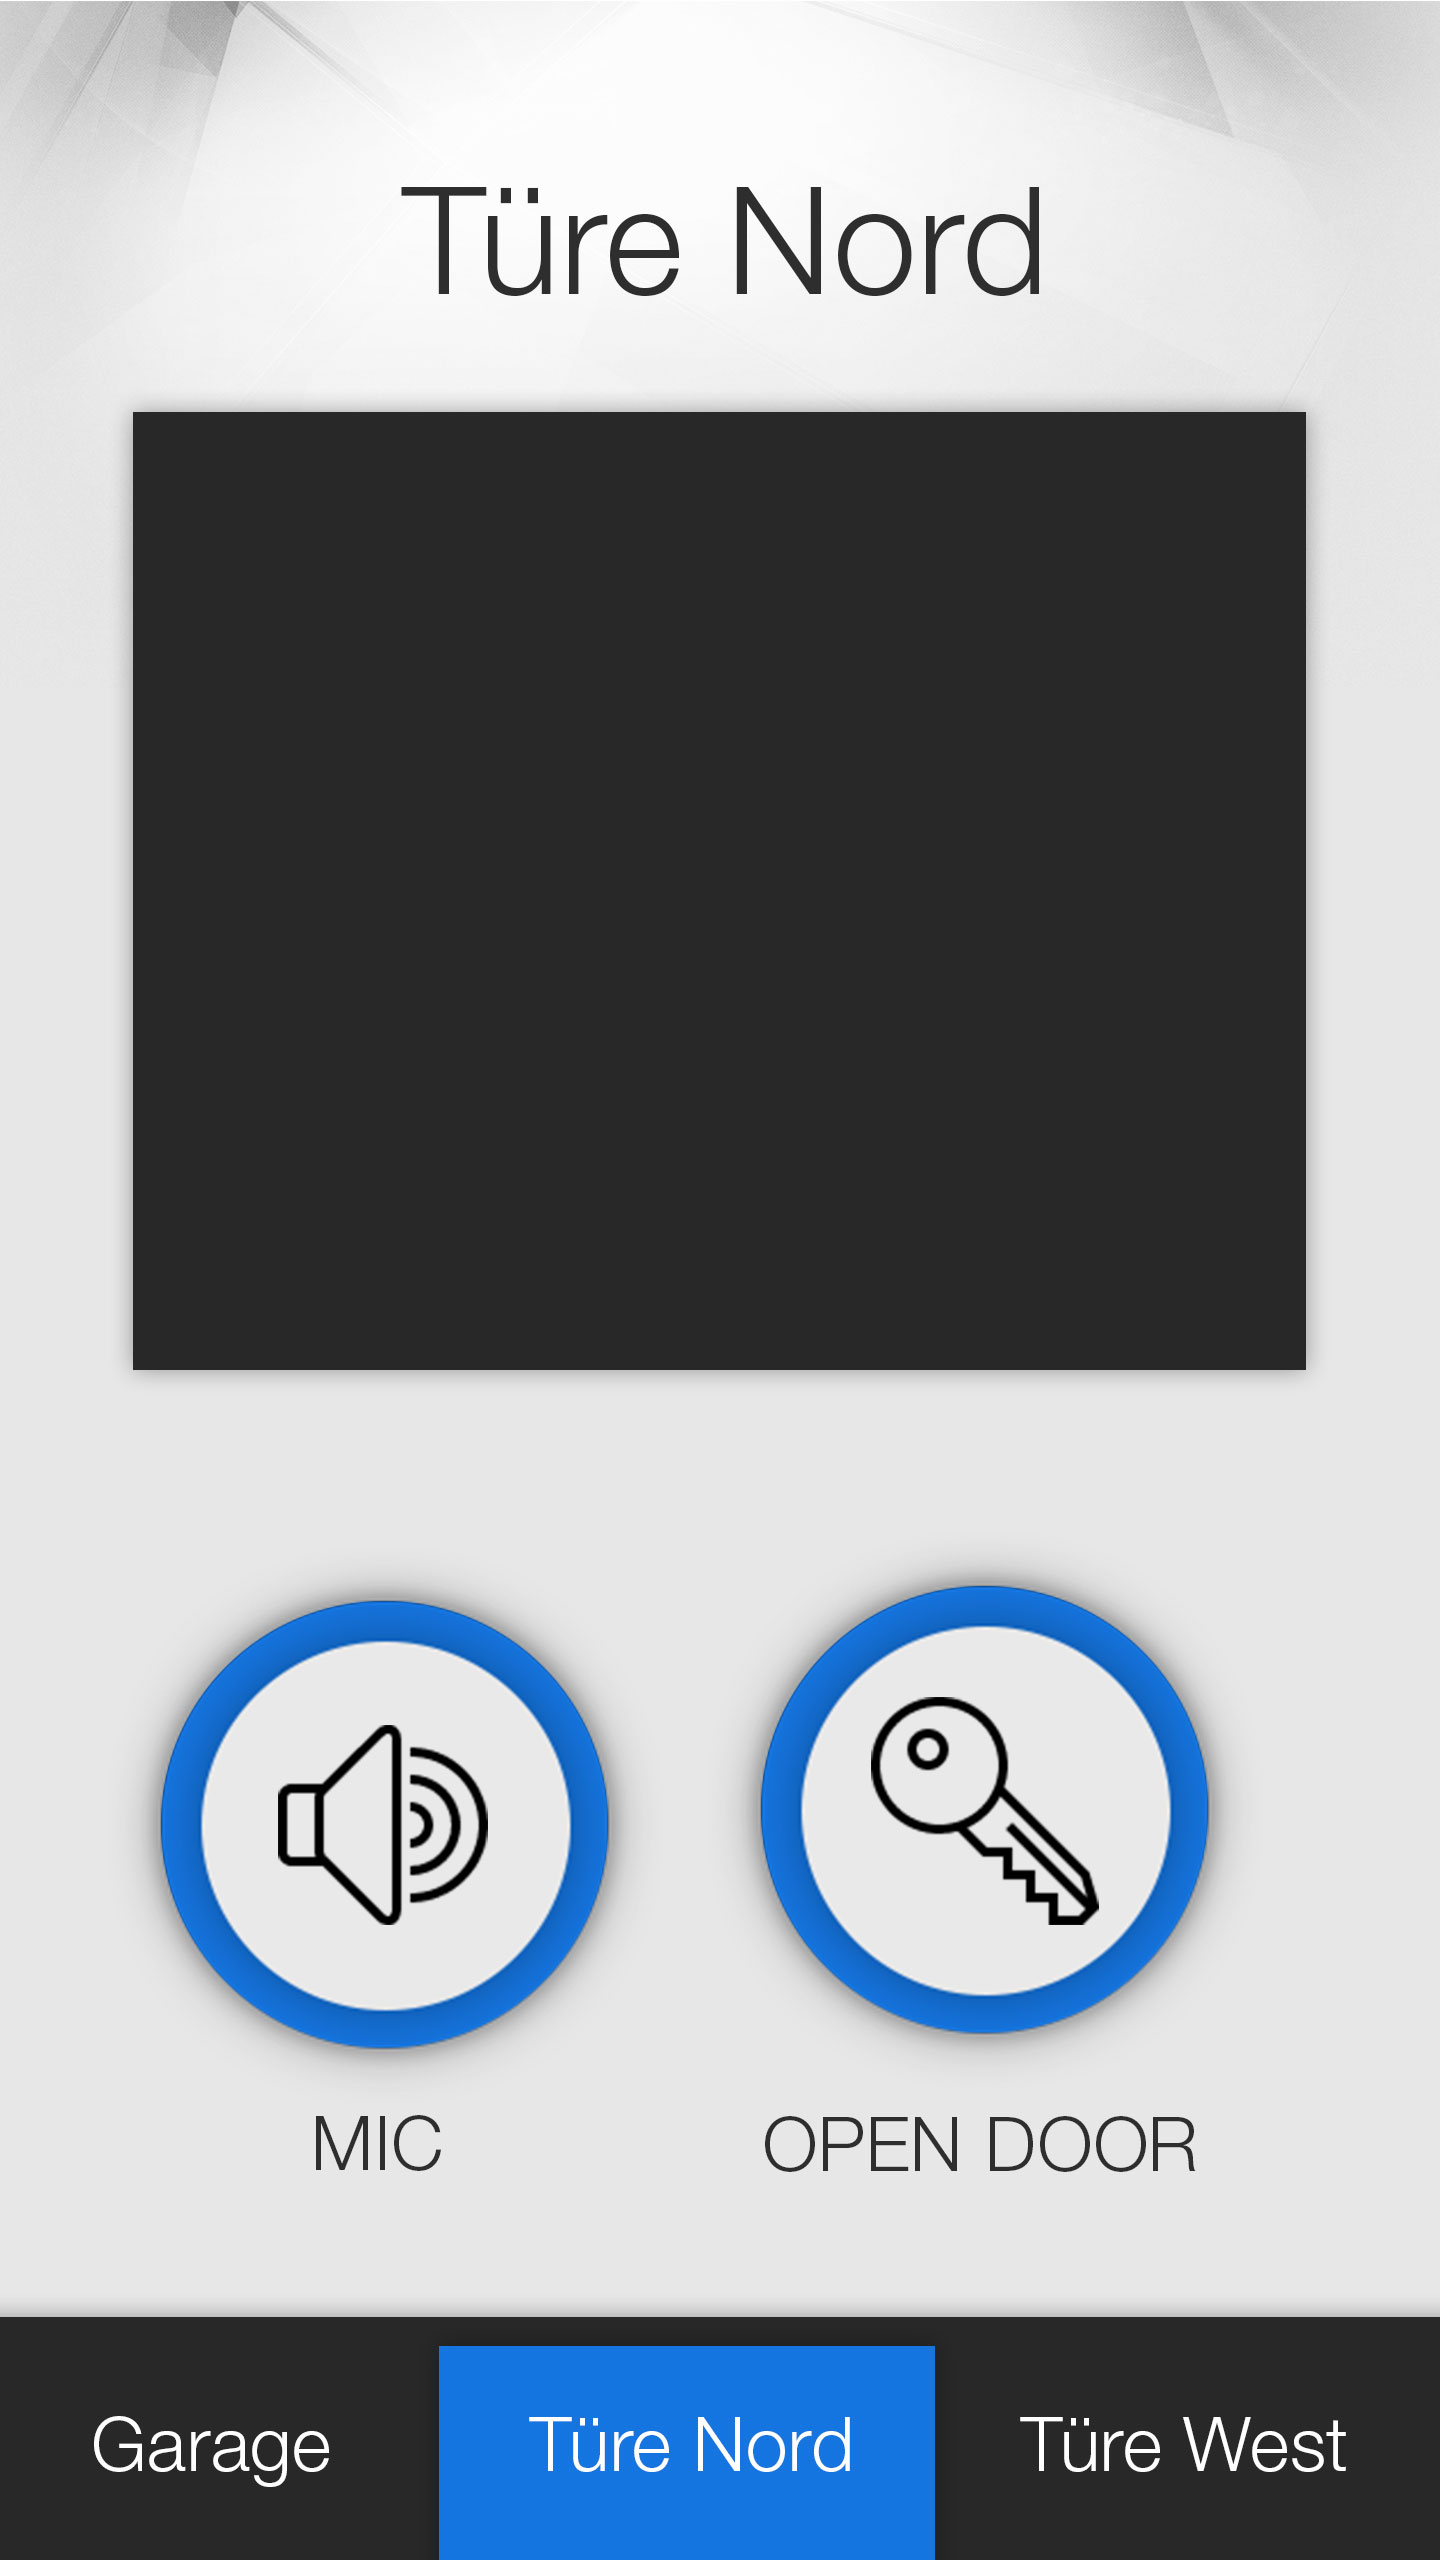
\includegraphics[width=0.35\textwidth]{clientDemo}
		\caption[Design der Client-Webapp]{Design der Client-Webapp}
		\label{fig:clientDemo}
	\end{center}
\end{figure}
\\
Die \cref{fig:clientDemo} zeigt das Design für die Webapplikation. Hier gezeigt ist die Smartphone Version. Dank ein Responsive-Design wird die selbe Applikation auch auf andere Geräte wie z.B. Tablets oder Computers passend angezeigt.
\\ 
Bei der Design-Entwurf standen Übersichtlichkeit und Benutzerfreundlichkeit im Vordergrund. Aus diesem Grund werden die Tasten für die Audio-Kommunikation und für die Öffnung der Türe gross Angezeigt. Das Videostream von der ausgewählte Türe wird sofort angezeigt und benötigt keine weitere Interaktion. 

\subsubsection{Aussensprechstelle Webapplikation}
..

\subsubsection{Management Tool}
\label{kap:managementtool}
Um eine schnellere Inbetriebnahme und eine zentrale Verwaltung des Systems zu gewährleisten, wurde der Management Tool etwickelt. Dieses Portal ermöglicht die Erfassung der Gegensprechanlagen und der Wohnungen.
Diese Schnitstelle wurde mit webtechnologien entwickelt(HTML, PHP, Js) und wird zusammen mit den MySQL Database auf den localen Raspberry Server gehostet. Aus Sicherheitsgründen werden alle eingehende und ausgehende Verbindungen abhörsicher aufgebaut.
\\
Grund dafür das einsetzten von Webtechnologien ist die Plattformunabhängigkeit sowie die Einfachkeit und die Standardisierung der Sprachen. Für den ersten Prototyp lag der Fokus auf die funktionale Eingenschaften der Tool. Bei einer zukünfitige Weiterentwicklung des Produkt kann man, dank der Webtechnologien mit gerigere Aufwand das Tool skalieren bzw. neue Features hinzufühgen.  

\begin{figure}[htb!]
	\begin{center}
		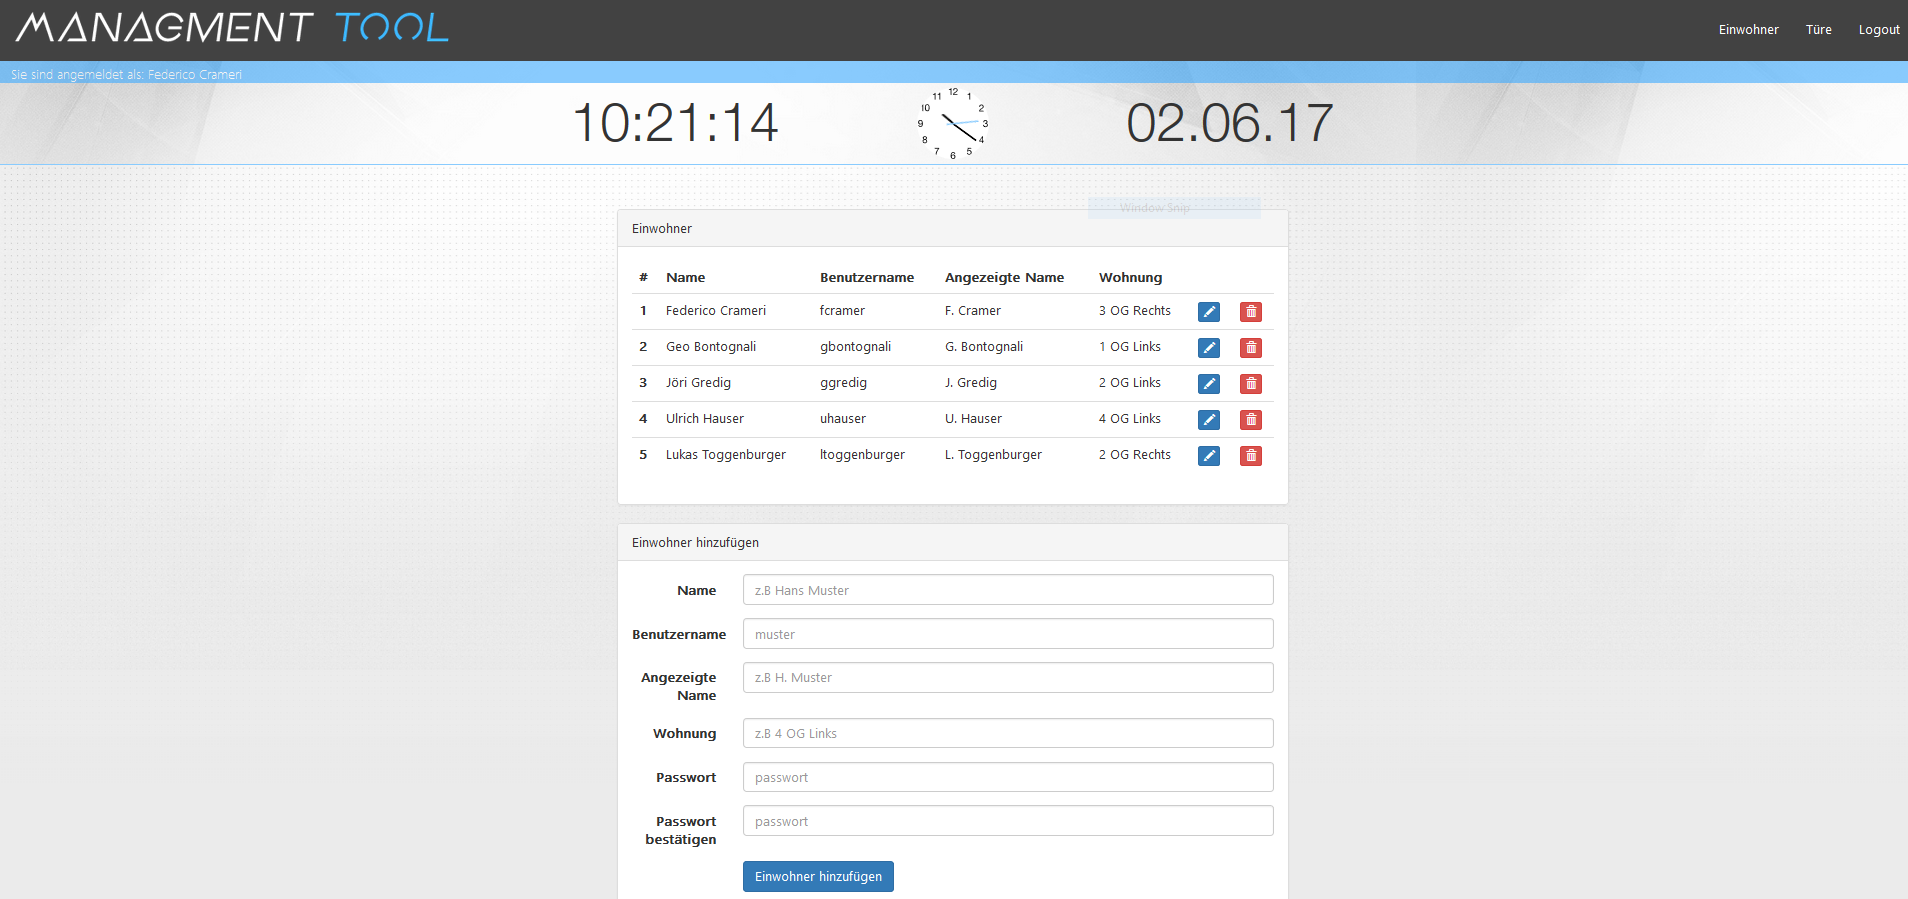
\includegraphics[width=1\textwidth]{managementtool}
		\caption[Design der Management tool]{Design der Management tool}
		\label{fig:managementtool}
	\end{center}
\end{figure}

Das Tool in mit ein Login versehen, somit ist sichergestellt das nur der Hausverwalter die Anlage verwalten kann. 
\subsubsection{Bewohner}
Unter die Bewohner Seite werden alle Wohnungen, beziehungsweise alle Bewohner aufgelistet. Diese verfühgen über ein Benutzername sowie eine Passwort die Von der Client App wervendet wird um sie sich bei den Server zu authentifizieren. Dieser Abschnitt bietet noch die Möglichkeit der Name und die Position der Wohnung welcher an den Aussensprechstelle ~\ref{fig:aussensprechstelle} angezeigt wird, abzuändern.
\subsubsection{Türen}
Bei der Einbau eine neue Tür, kann diese in dem Management Tool aufgeführt werden. Dabei muss beachtet werden dass der Id mit derjenige die auf den neu installierte Aussensprechstelle übereinstimmt. In diese Sektion sind auch die Namen der Türen definiert, welche denn auf den Client App (Siehe Abbildung ~\ref{fig:managementtool})  angezeigt werden. 


\subsection{Remote Verbindung}
\label{kap:remote}
..

\subsection{WebRTC}
\label{kap:webrtc}
WebRTC ist ein offener Standard, der eine Sammlung von Kommunikationsprotokollen und API beinhaltet. Die Standardisierung wird mehrheitlich betrieben und unterstützt von Google, Mozilla Foundation und Opera Software. WebRTC basiert auf HTML5 und Javascript und die Audio/Video Übertragung erfolgt über eine direkte Verbindung zwischen den Sprechpartner (Peer-to-Peer).
\\
\\
WebRTC wird hauptsächlich für die Entwicklung von Videokonferenz Programme verwendet. Die Natur dieses Projekt ist allerdings nicht dieselbe wie die herkömmliche Real-Time-Communication Applikationen. Glücklicherweise wurde WebRTC so entwickelt, um möglichst viel Flexibilität zu garantieren. Aus diesem Grund beinhaltet der WebRTC-Standard keine Definition für den Signaling-Process, welcher zusammen mit dem ICE (Interactive Connectivity Establishment) für den Verbindungsaufbau zwischen den Sprechpartnern zuständig ist. 

\begin{quote}
	\textit{
		"The thinking behind WebRTC call setup has been to fully specify and control the media plane, but to leave the signaling plane up to the application as much as possible. The rationale is that different applications may prefer to use different protocols, such as the existing SIP or Jingle call signaling protocols, or something custom to the particular application, perhaps for a novel use case. [...]"
	} 
	\\
	\cite[Sam Dutton, HTML5Rocks.com]{001} 
\end{quote}

\subsubsection{Signaling Process}
\label{kap:signaling}

Ähnlich wie bei VoIP-Telefonie \textit{(SIP)}, brauchen die Sprechpartner ein gemeinsam bekanntes Knoten, um die Verbindung zu initialisieren (\seeref{fig:signaling}). In den meisten Fällen ist einem Partner, die logische Adressierung der andere Partner nicht bekannt. Es besteht also keine Möglichkeit um eine P2P Verbindung auf einmal zu starten.
\begin{figure}[htb!]
	\begin{center}
		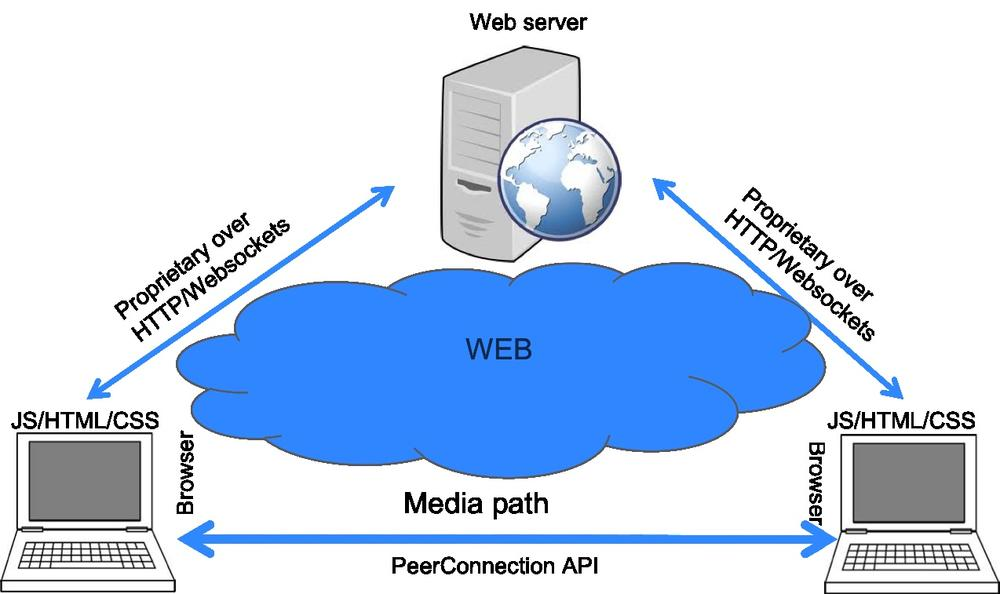
\includegraphics[width=0.75\textwidth]{signalingprocess}
		\caption[Der Signaling Prozess]{Der Signaling Prozess}
		\label{fig:signaling}
	\end{center}
\end{figure}
\\
Im unseren Fall wäre es theoretisch möglich, da die Position der Aussensprechstellen bzw. der Server immer dieselbe sind. Allerdings wurde WebRTC nicht so konzipiert. Die Standard WebRTC API beinhaltet kein Konstrukt um eine Verbindung anhand von Bekannter IP-Adresse aufbauen zu können.
\\
Im Internet sind es mehrere Signaling-Server Libraries verfügbar. Allerdings sind diese für andere Anwendungen gedacht. Im unseren System, wird beispielsweise nie eine Anruf von der Aussensprechstelle zu den Client-App gestartet, sondern lediglich umgekehrt.
\\
Für die Zwecke unser Projekt wurde ein eigenes Signaling-Server entwickelt. Dieser wird auf den Server ausgeführt und somit bleibt der Datenverkehr zwischen dem Client-App und der Aussensprechstelle, während jeder Schritt der Verbindungsaufbau und Kommunikation, innerhalb des lokales Netzwerkes. Das natürlich nur, solange der Bewohner sich zu Hause befindet.

\subsubsection{STUN Servers \& Remote Verbindung}
\label{test}
Eine Anforderung des Systems ist die Möglichkeit, auch ausserhalb des Heimnetzes mit den Aussensprechstellen sich verbinden zu können. Hier stellt das NAT-Protokoll (Network Adress Translation) ein Problem dar.
\\
Nach dem Signaling-Prozess wird das ICE-Prozess gestartet. Hier tauschen sich die zwei Partner Informationen über die eigene Adressierung und den \textit{best path} aus. Falls sich ein Sprechpartner hinter ein NAT-Knote befindet, wird für den anderen unmöglich sein eine Verbindung aufzubauen. Hier kommen die STUN-Servers im Spiel. Ähnlich wie bei dem Signalisierungsprozess stehen STUN-Servers als Hilfe für den Verbindungsaufbau da (\seeref{fig:stun}).
\begin{figure}[htb!]
	\begin{center}
		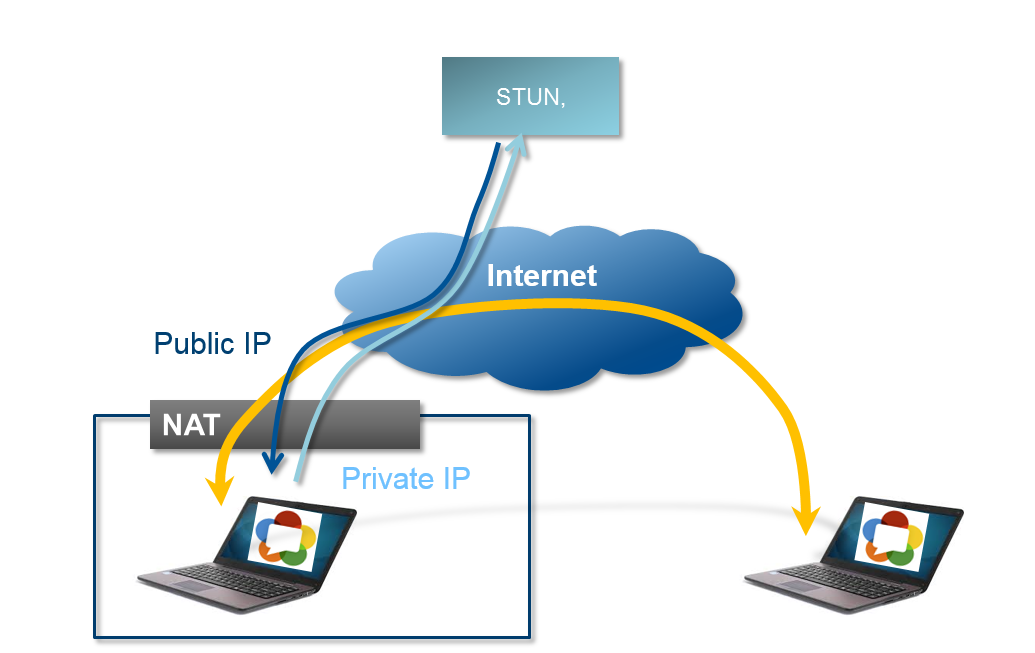
\includegraphics[width=0.75\textwidth]{stun}
		\caption[STUN Server]{STUN Server}
		\label{fig:stun}
	\end{center}
\end{figure}
 STUN-Servers informieren die Clients über jegliche NAT Konfigurationen die sich dazwischen befinden würden. Die beide Sprechpartner erhalten somit Informationen über welche Ports und Öffentliche Adressen die Verbindung initialisiert werden kann. Für die Entwicklung dieses Projektes werden die Google STUN Servers verwendet, welche kostenfrei zur Verfügung stehen.
\\
Falls sich beide Sprechpartner im gleichen lokales Netzwerk befinden, werden keine STUN-Servers benötigt und den gesamten Datenverkehr bleibt innerhalb des Heimnetzwerkes.

\newpage







%%Verzeichnis aller Bilder


%%Literaturverzeichnis
\newpage
\bibliography{lit}
\bibliographystyle{plain}
\addcontentsline{toc}{section}{Literaturverzeichnis}
\newpage

%% Abbildungsverzeichnis, Tabellenverzeichnis, Abkürzungsverzeichnis
\listoffigures
\addcontentsline{toc}{section}{Abbildungsverzeichnis}
\newpage
\listoftables
\addcontentsline{toc}{section}{Tabellenverzeichnis}
\newpage

\thispagestyle{plain}
\section*{Abkürzungsverzeichnis}
\addcontentsline{toc}{section}{Abkürzungsverzeichnis}
\newpage
\thispagestyle{plain}

%\begin{center}
%\begin{minipage}[t]{1\textwidth}
\section*{Eidesstattliche Erklärung}
\addcontentsline{toc}{section}{Eidesstattliche Erklärung}
Die Verfasser dieser Bachelorarbeit, Fabiano Sala und Gabriel Salkim, bestätigen, dass sie die Arbeit selbstständig und nur unter Benützung der angeführten Quellen und Hilfsmittel angefertigt haben. Sämtliche Entlehnungen sind durch Quellenangaben festgehalten.
	
	
\vspace{2cm}

\hspace{2cm} Ort, Datum \hfill Gabriel Salkim \hspace{2cm}

\vspace{4cm}

\hspace{2cm} Ort, Datum \hfill Fabiano Sala \hspace{2cm}
%\end{minipage}
%\end{center}






% leere Seite einfügen
\thispagestyle{empty}
\quad 
\newpage

\end{document}
% ======================================= Dokumentende =======================================